\documentclass[14pt,a4paper]{extarticle}
\usepackage[utf8]{inputenc}

\usepackage[english,russian]{babel}
\usepackage{indentfirst}
\usepackage{amsmath}
\usepackage{amsfonts}
\usepackage{amssymb}
\usepackage{color}
\usepackage{float}
\usepackage{placeins}
\usepackage{mathrsfs}

\numberwithin{equation}{section}


\usepackage[version=3]{mhchem}% Package for chemical equation typesetting
%\renewcommand{\thefigure}{\thechapter.\Alph{figure}}


\usepackage{lineno}

%\linenumbers

\usepackage[usenames,dvipsnames,svgnames,table]{xcolor}
\usepackage[hypcap]{subcaption}
% \usepackage[colorlinks=true, linkcolor=Maroon, citecolor=ForestGreen]{hyperref}
\usepackage[colorlinks=false]{hyperref}
\usepackage{graphicx}
\usepackage{subcaption}
\usepackage[height=25cm, a4paper, hmargin={2.5cm, 1.5cm}, vmargin={2cm, 2.3cm}]{geometry}
\setlength{\parindent}{1em}
\setlength{\parskip}{0pt}% {.3em}

\usepackage{titlesec}
\titleformat*{\section}{\normalsize\bfseries}
\titleformat*{\subsection}{\normalsize\bfseries}
%\titlelabel{\thetitle.\quad}


\usepackage[separate-uncertainty = true, multi-part-units=single, range-phrase=--, range-units=single]{siunitx}

%\mathchardef\period=\mathcode`.
%\DeclareMathSymbol{.}{\mathord}{letters}{"3B}

\usepackage{setspace}
\onehalfspacing

\usepackage[backend=bibtex, style=numeric, sorting=none, maxnames=3, minnames=3, hyperref=true, url=true, isbn=false, backref=true]{biblatex}
\bibliography{mybib}

\usepackage{tocloft}
\usepackage{tikz}
\hyphenation{Ha-ma-ma-tsu}

%\newcommand{\RNum}[1]{\uppercase\expandafter{\romannumeral #1\relax}}

\usepackage{titletoc}
\dottedcontents{section}[3em]{}{2.9em}{1pc}
\dottedcontents{subsection}[3em]{}{2.3em}{1pc}
%\renewcommand{\thesection}{\thechapter\arabic{section}}
%\renewcommand{\thesection}{\thechapter\arabic{subsection}.}

\renewcommand{\figurename}{Рис.}
%\usepackage[labelsep=period, font=small]{caption}

\usepackage{titlesec}
\usepackage{physics}
\titlespacing*{\section}
{0pt}{1pt}{0pt}
% {0pt}{5.5ex plus 1ex minus .2ex}{4.3ex plus .2ex}
\titlespacing*{\subsection}
{0pt}{1pt}{0pt}
% {0pt}{5.5ex plus 1ex minus .2ex}{4.3ex plus .2ex}

\usepackage{fancyhdr}

\pagestyle{fancy}
\fancyhf{}
%\fancyhead[LE,RO]{Share\LaTeX}
%\fancyhead[RE,LO]{Guides and tutorials}
%\fancyfoot[CE,CO]{\leftmark}
\fancyfoot[LE,RO]{\thepage}
\renewcommand{\headrulewidth}{0pt}
\DeclareMathOperator{\sinc}{sinc}

\usepackage{datatool}
\usepackage{siunitx}
\usepackage{booktabs} % for nicer tables
\usepackage{caption} % improve caption spacing (among other things)
\usepackage{bm}
\renewcommand*\dtldisplaystarttab{\toprule}
\renewcommand*\dtldisplayendtab{\tabularnewline\bottomrule}
\renewcommand*\dtldisplayafterhead{\midrule}

\usepackage{pgfplotstable}
\usepackage{siunitx}
\usepackage{booktabs}

\begin{document}
	
	\section{Отчёт по техническому заданию для станции 1-1. Итерация 1.}
	\subsection{Входные параметры моделирования}
	Расчёт производился в SRW, версия для Python. Ссылка на GitHub SRW @O.Chubar \textit{\href{https://github.com/ochubar/SRW.git}{здесь}} , расчёты для каждого отдельно бимлайна хранятся в соответствующих репозиториях на GitHub, {\href{https://github.com/TrebAndrew/thesis_andrei.git}{ссылка}}. Входные параметры смотреть на гугл диске оптической группы, {\href{https://drive.google.com/open?id=1zY-qElVNPh--SjBYmQvyMo7WluX_Am-s}{ссылка}}. Остальное описание выполняемого технического задания дано в этом отчёте\\
	Автор: Требушинин Андрей; trebandrej@gmail.com
	\subsection{Задача №1}
	\textit{Источник - СП ондулятор (параметры ондулятора во вложении, параметры электронного пучка актуализировать у отв. лиц). Оценить размеры и расходимость источника для рабочих гармоник (11-й, 13-й, 17-й и 23-й)}\\
	%См. рис.~\ref{fig:before_crystal}
	Расчёт производился при параметрах электронного пучка см.таб.~\ref{table:ebeam}. Геометрические и угловые размеры излучения см. таб.~\ref{table:size_obeam}\\
	\begin{table}[h!]
		\centering
		\begin{tabular}{cccccccc}
			\hline
			\toprule
			\rule{0pt}{3ex}   $\sigma_x, [m]$ & $\sigma_{x'}, [rad]$ & $\sigma_y, [m]$     & $\sigma_{y'}, [rad]$ \\ \hline
			\rule{0pt}{3ex}   $33.0 \times 10^{-6}$  & $2.65 \times 10^{-6}$  &  $8.6 \times 10^{-7}$ & $5.0 \times 10^{-7}$   \\
			\hline	\hline
			\rule{0pt}{3ex}   $\Delta E / E$ & $\beta_x,[m]$ & $\beta_y,[m]$   & $I,[mA]$\\ \hline
			\rule{0pt}{3ex}	 $8.6 \times 10^{-4}$ & $12.49$ & $1.99$ & $400$ \\ \hline
			\toprule
			\rule{0pt}{4ex}
		\end{tabular}
		\caption{Пространственные и угловые размеры электронного пучка. Бета функция. Ток}
		\label{table:ebeam}
	\end{table}
	
	\DTLloaddb
	[
	noheader,
	keys={},
	headers={
		\shortstack{$n_{harm}$},
		\shortstack{$\sigma_x, [mm]$},
		\shortstack{$\sigma_y, [mm]$},
		\shortstack{$\sigma_x, [\mu rad]$},
		\shortstack{$\sigma_y, [\mu rad]$}}
	]
	{RMS_before}{tabl/RMS_before.csv}
	\begin{table}[h!]
		\sisetup{
			parse-numbers   = false,
			table-number-alignment = right,
			table-figures-integer = 4,
			table-figures-decimal = 4,
			input-decimal-markers = .
		}
		\renewcommand*\dtlrealalign{S}
		\caption{Сечение пучка на входе в первую апертуру (25 м)}
		\centering
		\DTLdisplaydb{RMS_before}
		\label{table:size_obeam}
	\end{table}
	
	\subsection{Задача №2}
	\textit{До первого окна пучок ограничивается прямоугольной апертурой, соответствующей $4\sigma$ сечения пучка по горизонтали и вертикали (рассчитать).}
	\begin{itemize}
		\item 	\textbf{Расстояние от источника}: $25$ m 
		\item 	\textbf{Апертура}: $4\sigma^{11 harm}_{x} \times 4\sigma^{11 harm}_{y}$
	\end{itemize}
	
	\subsection{Задача №3}
	\textit{Далее до выхода из фронт-энда пучок проходит через алмазные окна. Рассчитать суммарную толщину окон из расчёта 1\% подавления первой рабочей гармоники 14,4 кэВ, тепловую мощность, рассеиваемую на окнах, оценить необходимость охлаждения окон.}\\
	Кривые поглощения см.рис~\ref{fig:bragg_T}.\\
	\textbf{Толщина окна:} $100\mu m$\\
	\textbf{Пропускание на 11-ой гармонике:} $T = 0.974 $\\
	
	\begin{figure}[h!]
		\centering  
		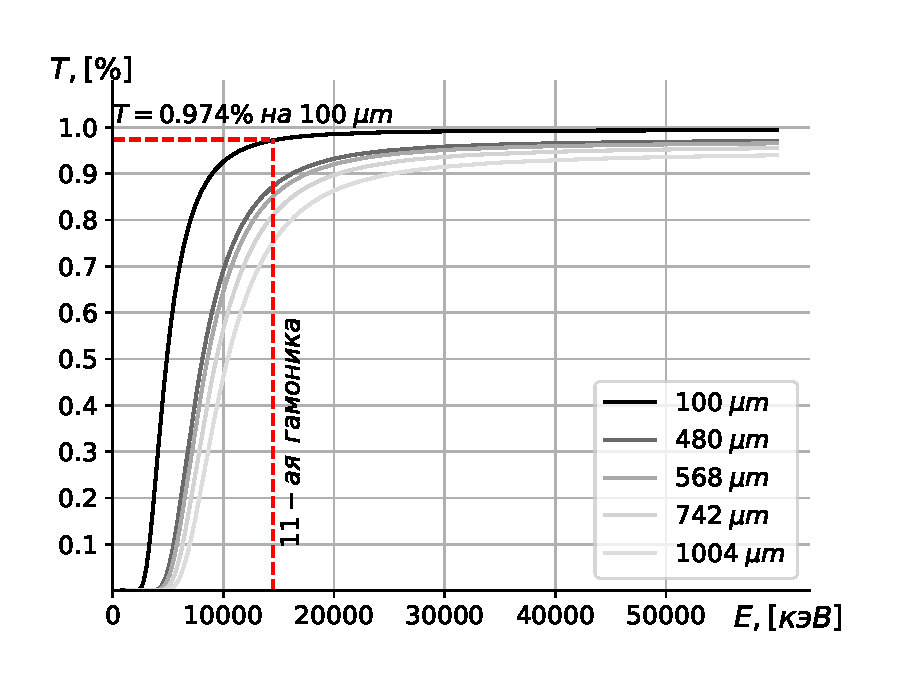
\includegraphics[width=\textwidth]{pic/bragg_T.pdf}	
		\caption{Кривые поглощения}
		\label{fig:absorb_spec}
	\end{figure}
	
	\subsection{Задача №4}
	\textit{Непосредственно за стеной фронт-энда (её положение актуализировать у отв. лиц) располагается оптический хатч, в котором максимально близко к фронт-энду (примерная схема во вложении) стоят подряд три алмазных бимсплиттера-монохроматора (Брэгг 111, толщина 100 мкм), отводящих в стороны пучки 11-й, 13-й и 23-й гармоник. Оценить размеры проекции пучка на рабочие поверхности монохроматоров, а также тепловую нагрузку и необходимость охлаждения.}\\
	На рис.~\ref{fig:OptScheme} представлена оптическая схема станции 1-1 для первой итерации. Тепловые нагрузки см. на рис.~\ref{fig:absorb_spec}, в таб.~\ref{table:stable} представлены данные по ориентации кристаллов.\\
	\newpage
	\begin{figure}[h!]
		\centering  
		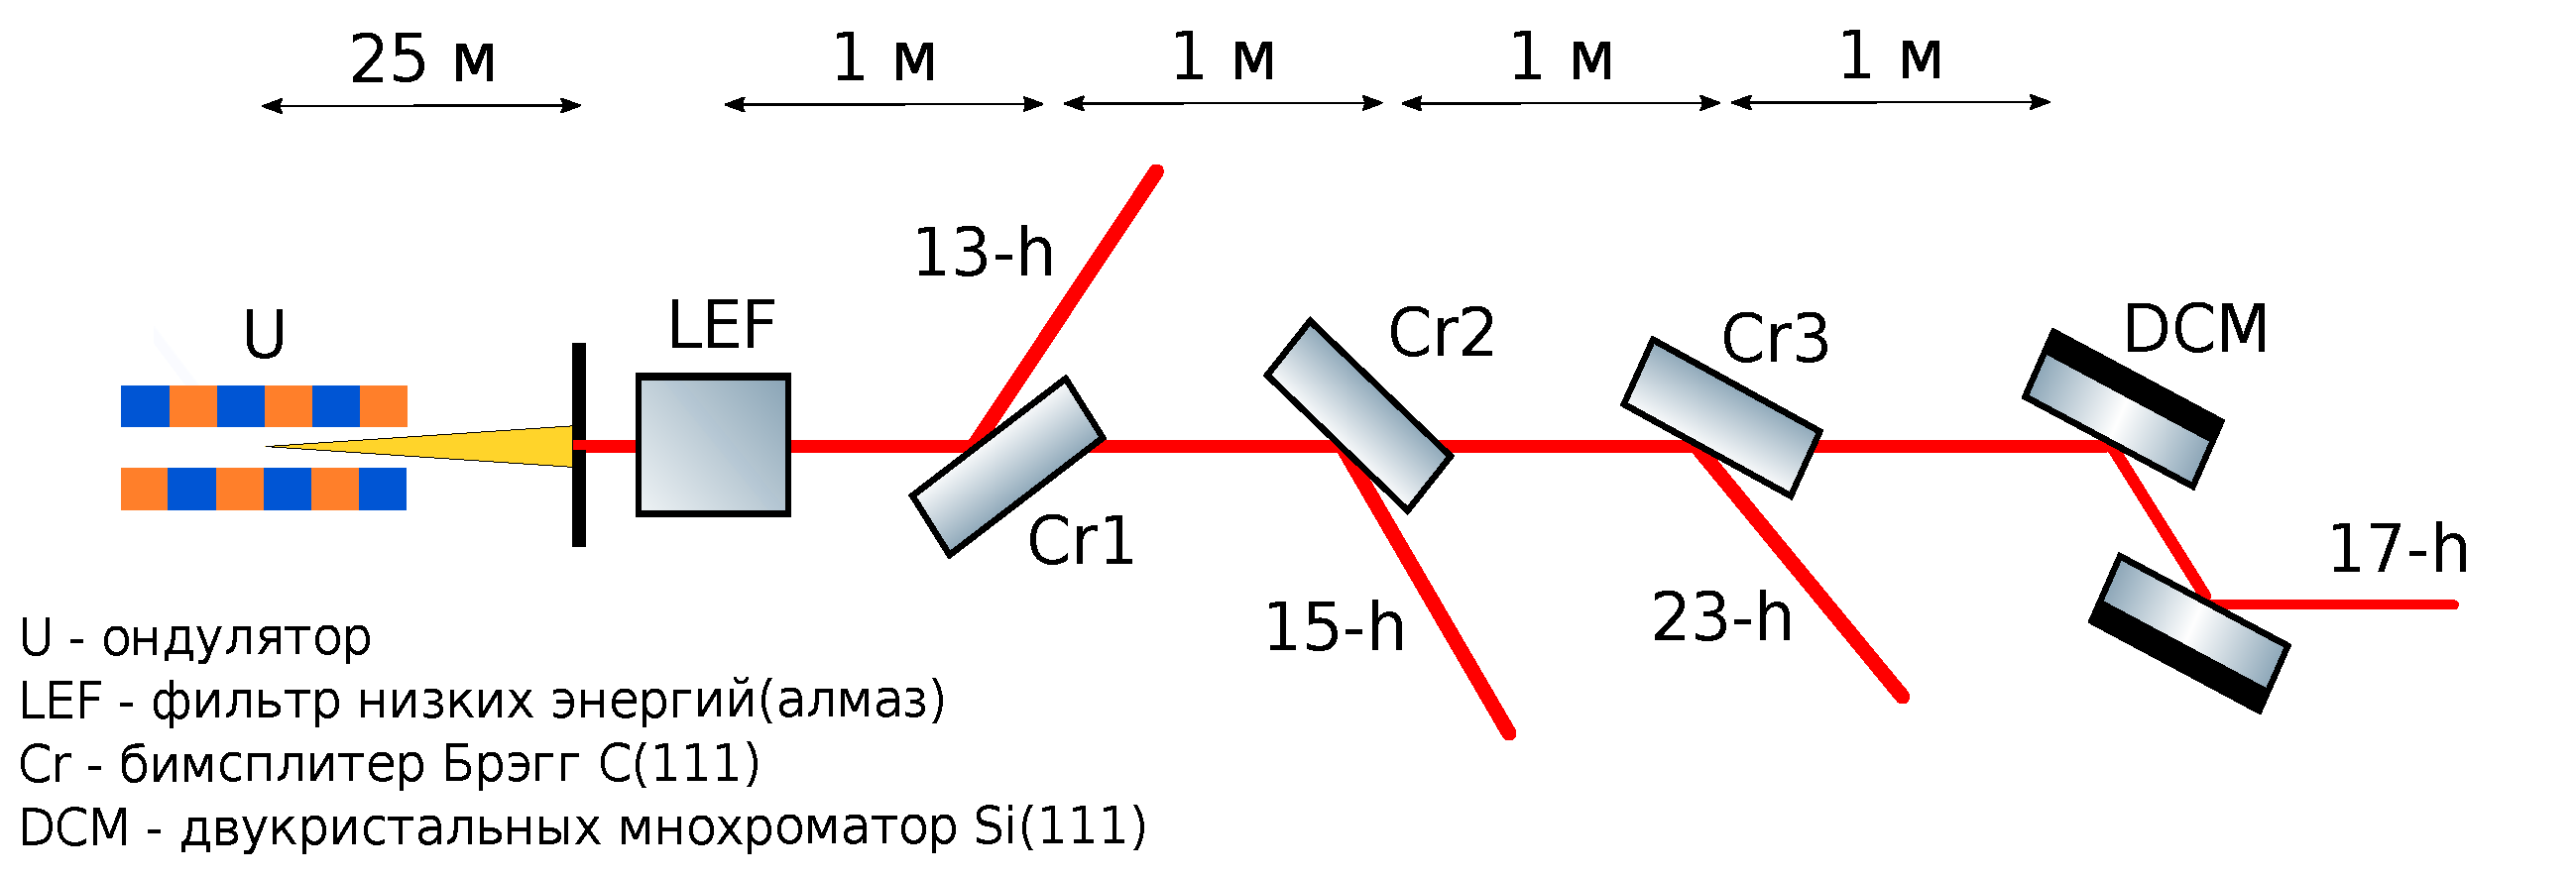
\includegraphics[width=\textwidth]{pic/OptScheme.pdf}
		\caption{Оптическая схема станции 1-1. Итерация 1.}
		\label{fig:OptScheme}
	\end{figure}

	\begin{figure}[h!]
		\centering  
		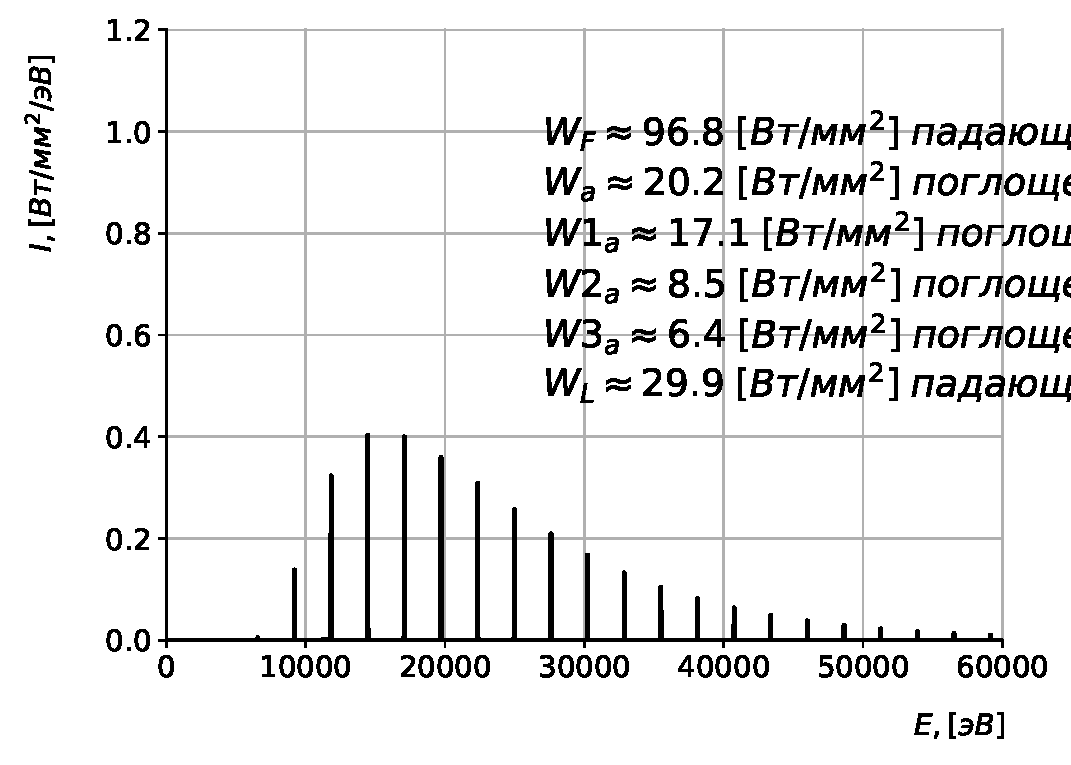
\includegraphics[width=\textwidth]{pic/spec.pdf}
		\caption{Розовый цвет --- падающая на алмазное окно спектральная мощность на оси. Чёрный цвет --- падающая спектральная мощность на DCM.}
		\label{fig:absorb_spec}
	\end{figure}

	\DTLloaddb
	[
	noheader,
	keys={},
	headers={
		\shortstack{$n_{harm}$},
		\shortstack{$\theta_{cr}, grad$},
		\shortstack{$d_{eff}, \mu m$},
		\shortstack{$S_{proj}, mm$}}
	]
	{Cr_angles}{tabl/Cr_angles.csv}
	\begin{table}[h!]
		\sisetup{
			parse-numbers   = false,
			table-number-alignment = right,
			table-figures-integer = 4,
			table-figures-decimal = 4,
			input-decimal-markers = .
		}
		\renewcommand*\dtlrealalign{S}
		\caption{Номер гармоники, ориентация кристалла, эффективная толщина CCM кристалла, проекция пучка(горизонтальная) }
		\centering
		\caption{Ориентация кристалла}
		\DTLdisplaydb{Cr_angles}
		\label{table:stable}
	\end{table}
	
	\subsection{Задача №5}
	\textit{Рассчитать сечение пучков, покидающих алмазные монохроматоры.}\\
	См.рис.~\ref{fig:after_crystal} и таб.~\ref{table:size_obeam_after}
	\DTLloaddb
	[
	noheader,
	keys={},
	headers={
		\shortstack{$n_{harm}$},
		\shortstack{$\sigma_x, [mm]$},
		\shortstack{$\sigma_y, [mm]$},
		\shortstack{$\sigma_x, [\mu rad]$},
		\shortstack{$\sigma_y, [\mu rad]$}}
	]
	{RMS_after}{tabl/RMS_after.csv}
	\begin{table}[h!]
		\sisetup{
			parse-numbers   = false,
			table-number-alignment = right,
			table-figures-integer = 4,
			table-figures-decimal = 4,
			input-decimal-markers = .
		}
		\renewcommand*\dtlrealalign{S}
		\caption{Сечение пучка после монохроматоров}
		\centering
		\DTLdisplaydb{RMS_after}
		\label{table:size_obeam_after}
	\end{table}
	
	\subsection{Задача №6}
	\textit{Рассчитать тепловую нагрузку оставшегося прямого пучка на двукристальный кремниевый 111 монохроматор, расположенный в удалённом хатче (см. схему), а также сечение пучка на выходе из монохроматора. Оценить необходимость и тип охлаждения.}\\
	Тепловые нагрузки см. на рис.~\ref{fig:absorb_spec}.
	\DTLloaddb
	[
	noheader,
	keys={},
	headers={
		\shortstack{$n_{harm}$},
		\shortstack{$E, eV$},
		\shortstack{$\lambda, [nm]$},
		\shortstack{$ph/s$},
		\shortstack{$ph/s/0.1\%$},
		\shortstack{$\Delta E / E$}}
	]
	{ph_beam_par_after_cr}{tabl/ph_beam_par_after_cr.csv}
	\begin{table}[h!]
		\sisetup{
			parse-numbers   = false,
			table-number-alignment = right,
			table-figures-integer = 4,
			table-figures-decimal = 4,
			input-decimal-markers = .
		}
		\renewcommand*\dtlrealalign{S}
		\caption{Потоки с выхода монохроматоров}
		\centering
		\DTLdisplaydb{ph_beam_par_after_cr}
	\end{table}
	
	\newpage
	\subsection{Дополнение. Кривые Дарвина для алмаза и кремния на рабочих гармониках}
	Кривые Дарвина для алмаза и кремния представлены на рис.~\ref{fig:Diamond_bragg_R} и~\ref{fig:Silicon_bragg_R}, соответственно.В таб.~\ref{table:Darvin_curve_diamond} и~\ref{table:Darvin_curve_silicon} даны FWHM этих кривых. 
	 
	\DTLloaddb
	[
	noheader,
	keys={},
	headers={
		\shortstack{$n_{harm}$},
		\shortstack{$FWHM, \mu rad$}}
	]
	{Darvin_curve_diamond}{tabl/Darvin_curve_diamond.csv}
	\begin{table}[h!]
		\sisetup{
			parse-numbers   = false,
			table-number-alignment = right,
			table-figures-integer = 4,
			table-figures-decimal = 4,
			input-decimal-markers = .
		}
		\renewcommand*\dtlrealalign{S}
		\caption{FWHM для алмаза}
		\centering
		\DTLdisplaydb{Darvin_curve_diamond}
		\label{table:Darvin_curve_diamond}
	\end{table} 

	\DTLloaddb
	[
	noheader,
	keys={},
	headers={
		\shortstack{$n_{harm}$},
		\shortstack{$FWHM, \mu rad$}}
	]
	{Darvin_curve_silicon}{tabl/Darvin_curve_silicon.csv}
	\begin{table}[h!]
		\sisetup{
			parse-numbers   = false,
			table-number-alignment = right,
			table-figures-integer = 4,
			table-figures-decimal = 4,
			input-decimal-markers = .
		}
		\renewcommand*\dtlrealalign{S}
		\caption{FWHM для кремния}
		\centering
		\DTLdisplaydb{Darvin_curve_silicon}
		\label{table:Darvin_curve_silicon}
	\end{table} 
	
	\begin{figure}[h!]
		\centering  
		\begin{minipage}{0.49\textwidth}
			\centering
			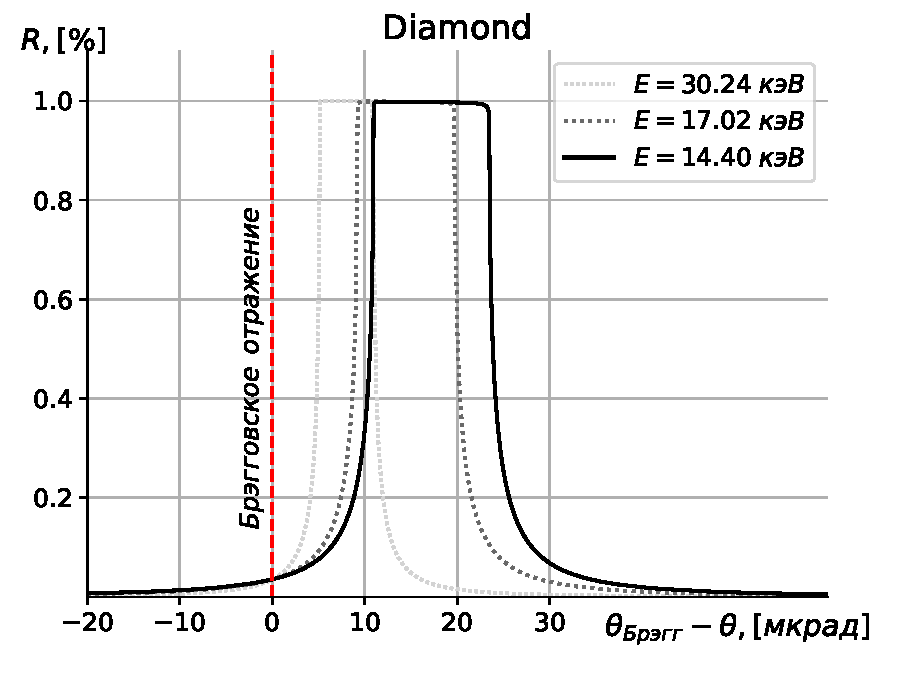
\includegraphics[width=\textwidth]{pic/Diamond_bragg_R.pdf}
			\caption{}
			\label{fig:Diamond_bragg_R}
		\end{minipage}\hfill
		\begin{minipage}{0.49\textwidth}
			\centering
			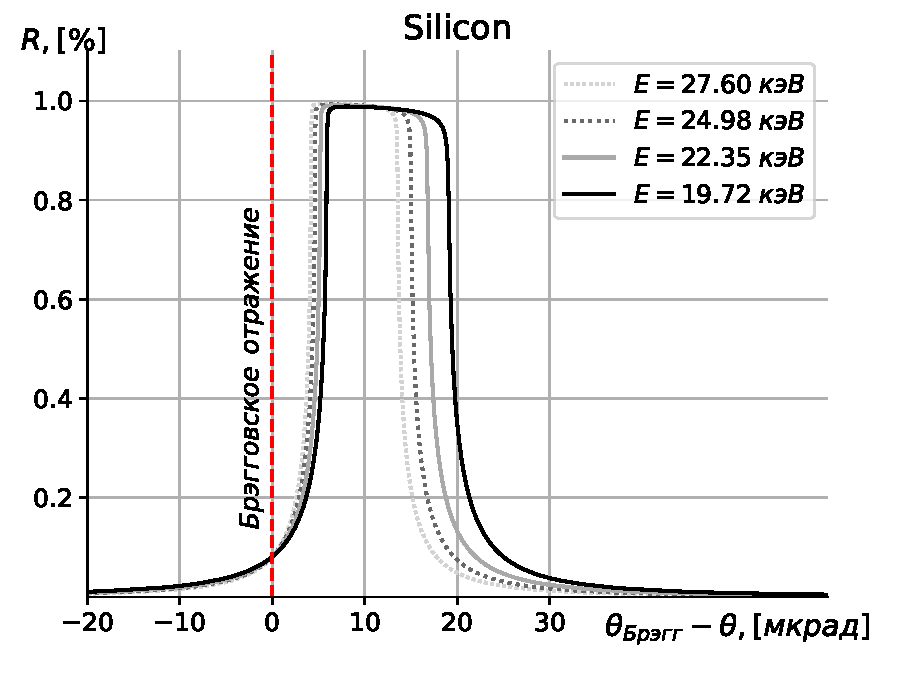
\includegraphics[width=\textwidth]{pic/Silicon_bragg_R.pdf}
			\caption{}
			\label{fig:Silicon_bragg_R}
		\end{minipage}    
	\end{figure}
	 		
	 \newpage
	\begin{figure}[htbp]
		\centering  
		\begin{minipage}{0.49\textwidth}
			\centering
			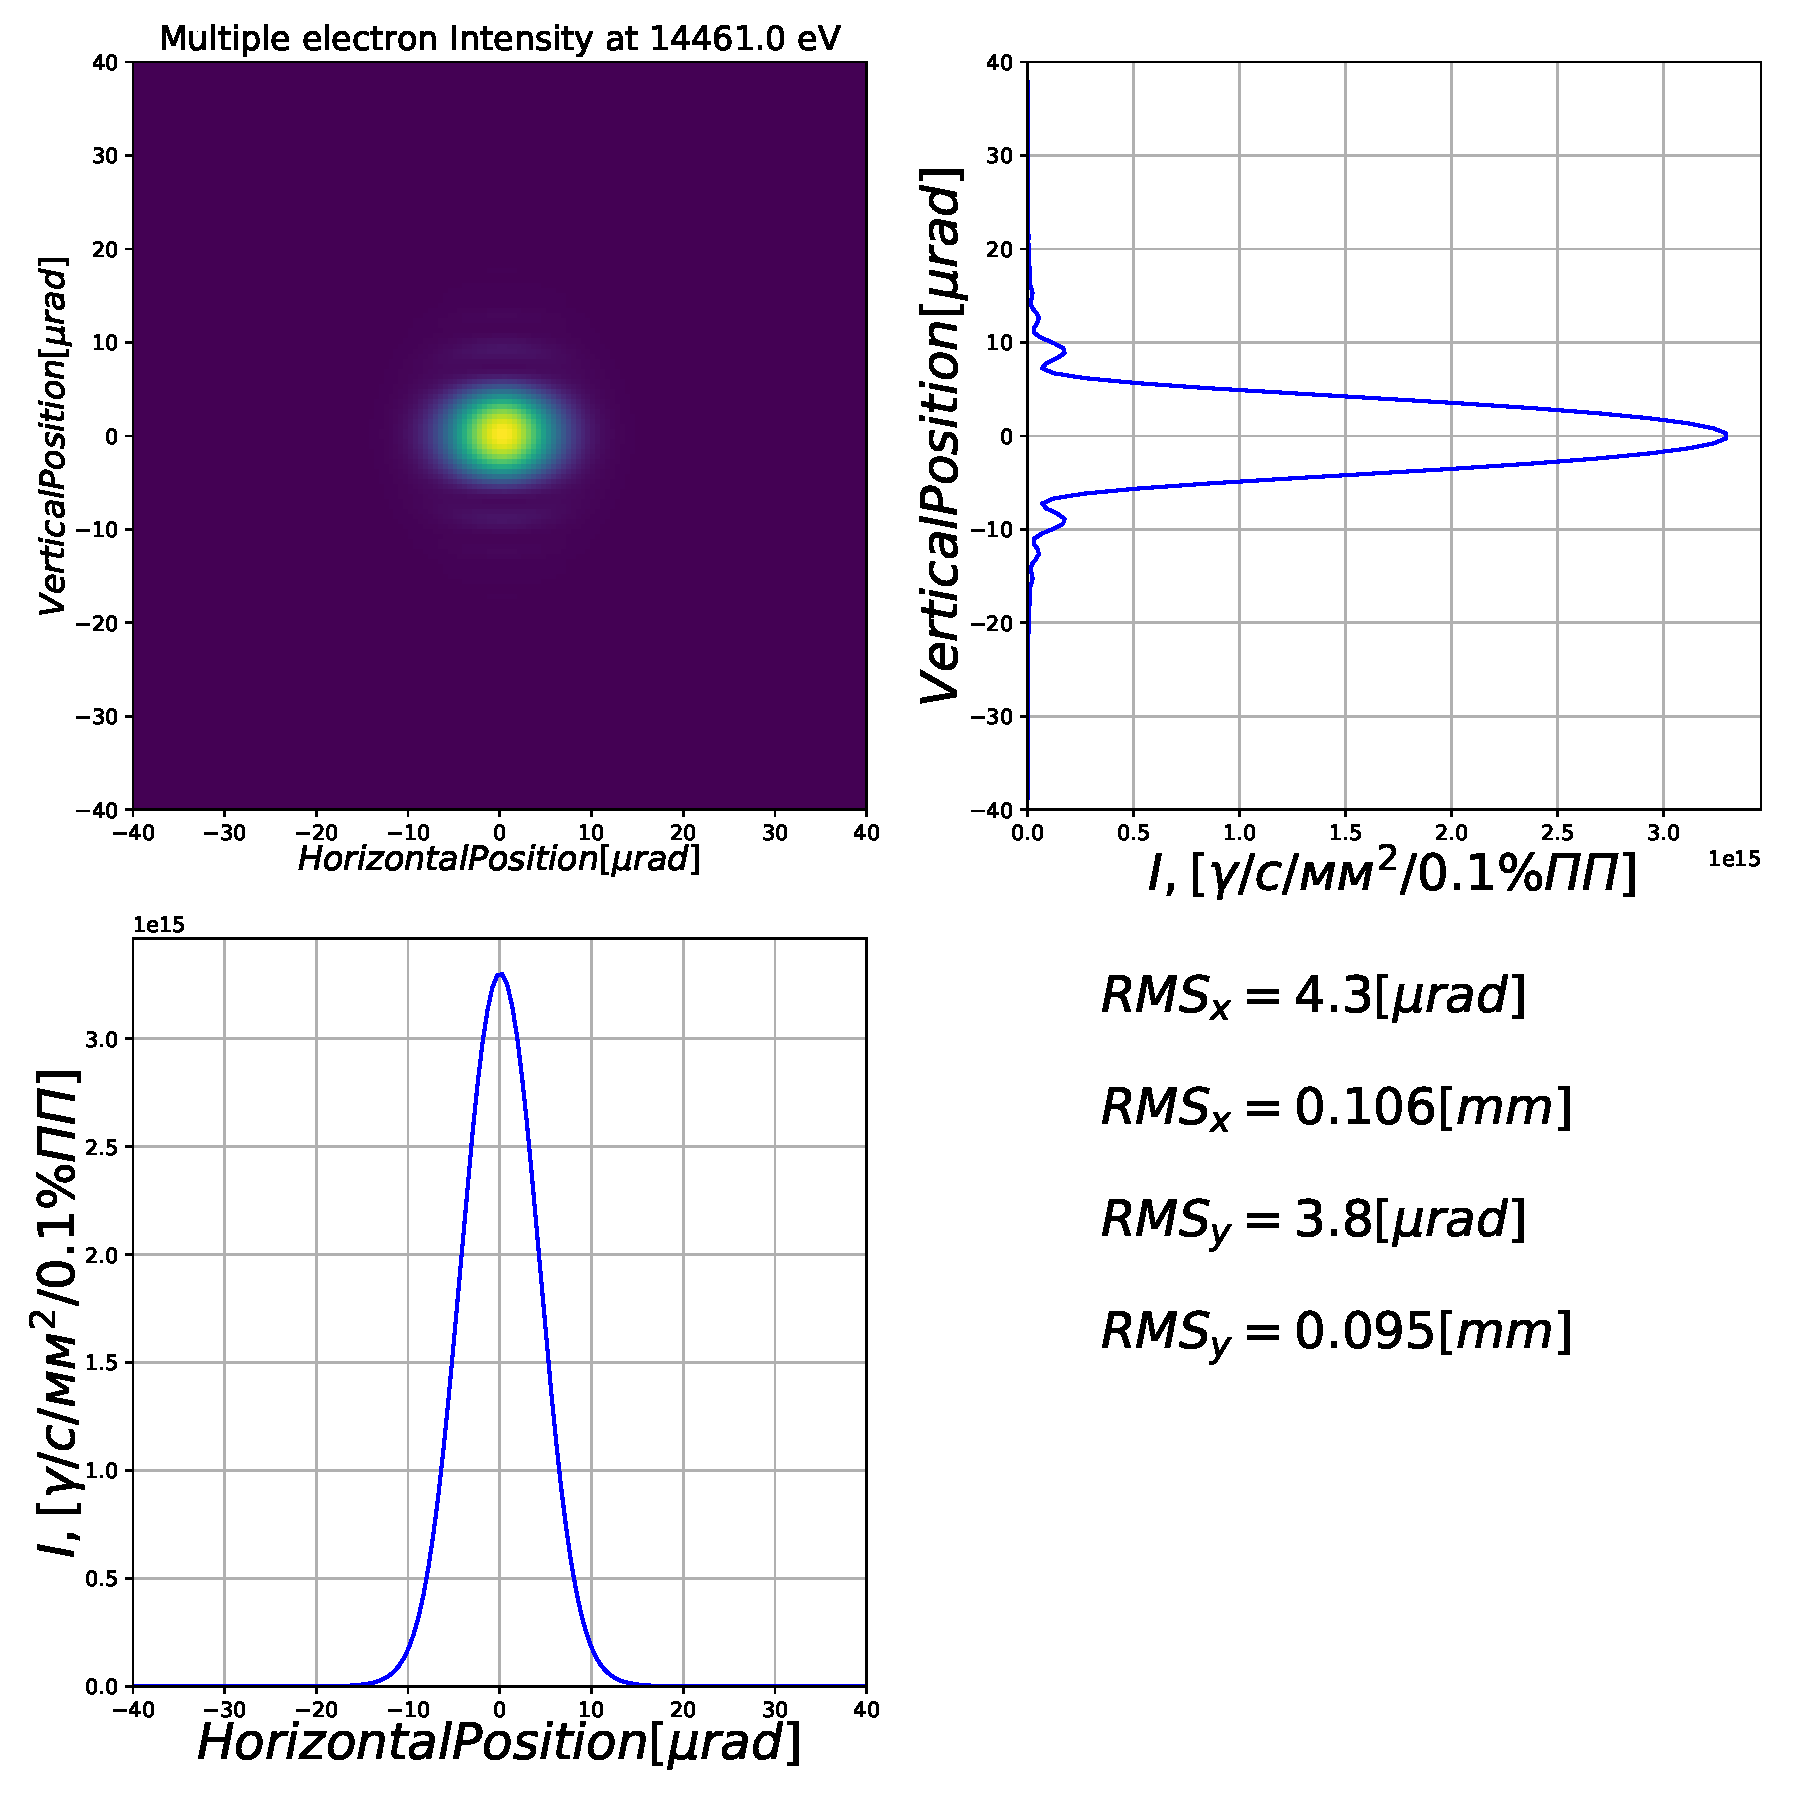
\includegraphics[width=\textwidth]{{pic/11_harm_before_crystal}.pdf}
		\end{minipage}\hfill
		\begin{minipage}{0.49\textwidth}
			\centering
			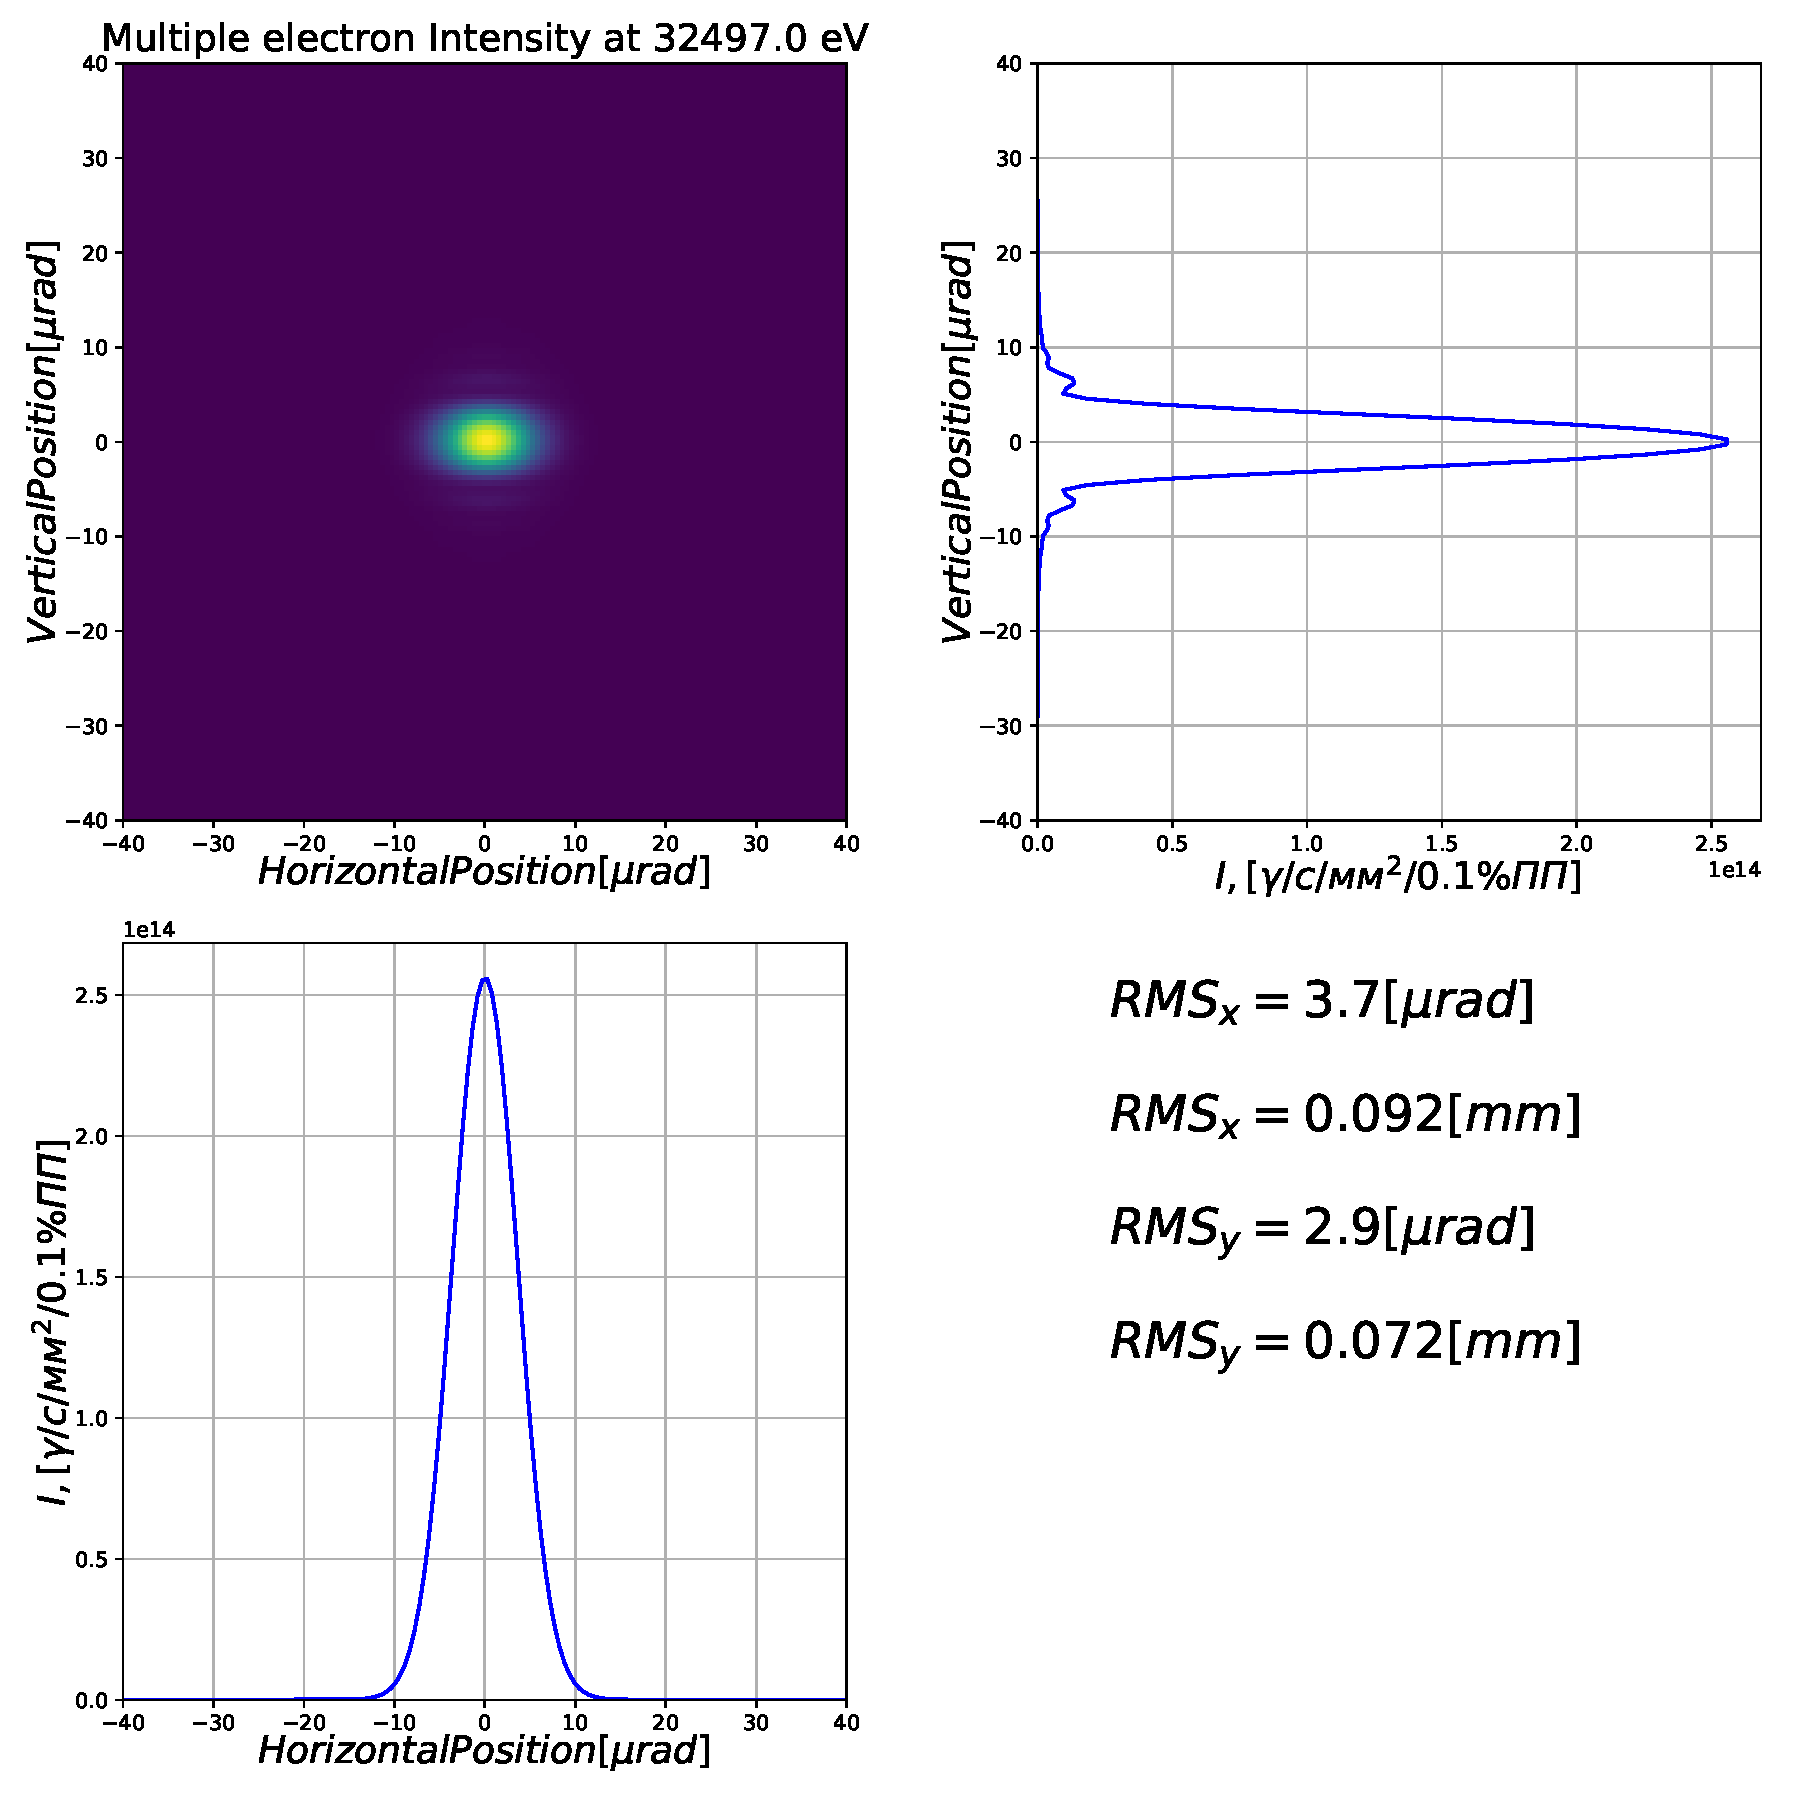
\includegraphics[width=\textwidth]{{pic/13_harm_before_crystal}.pdf}
		\end{minipage}
		\begin{minipage}{0.49\textwidth}
			\centering
			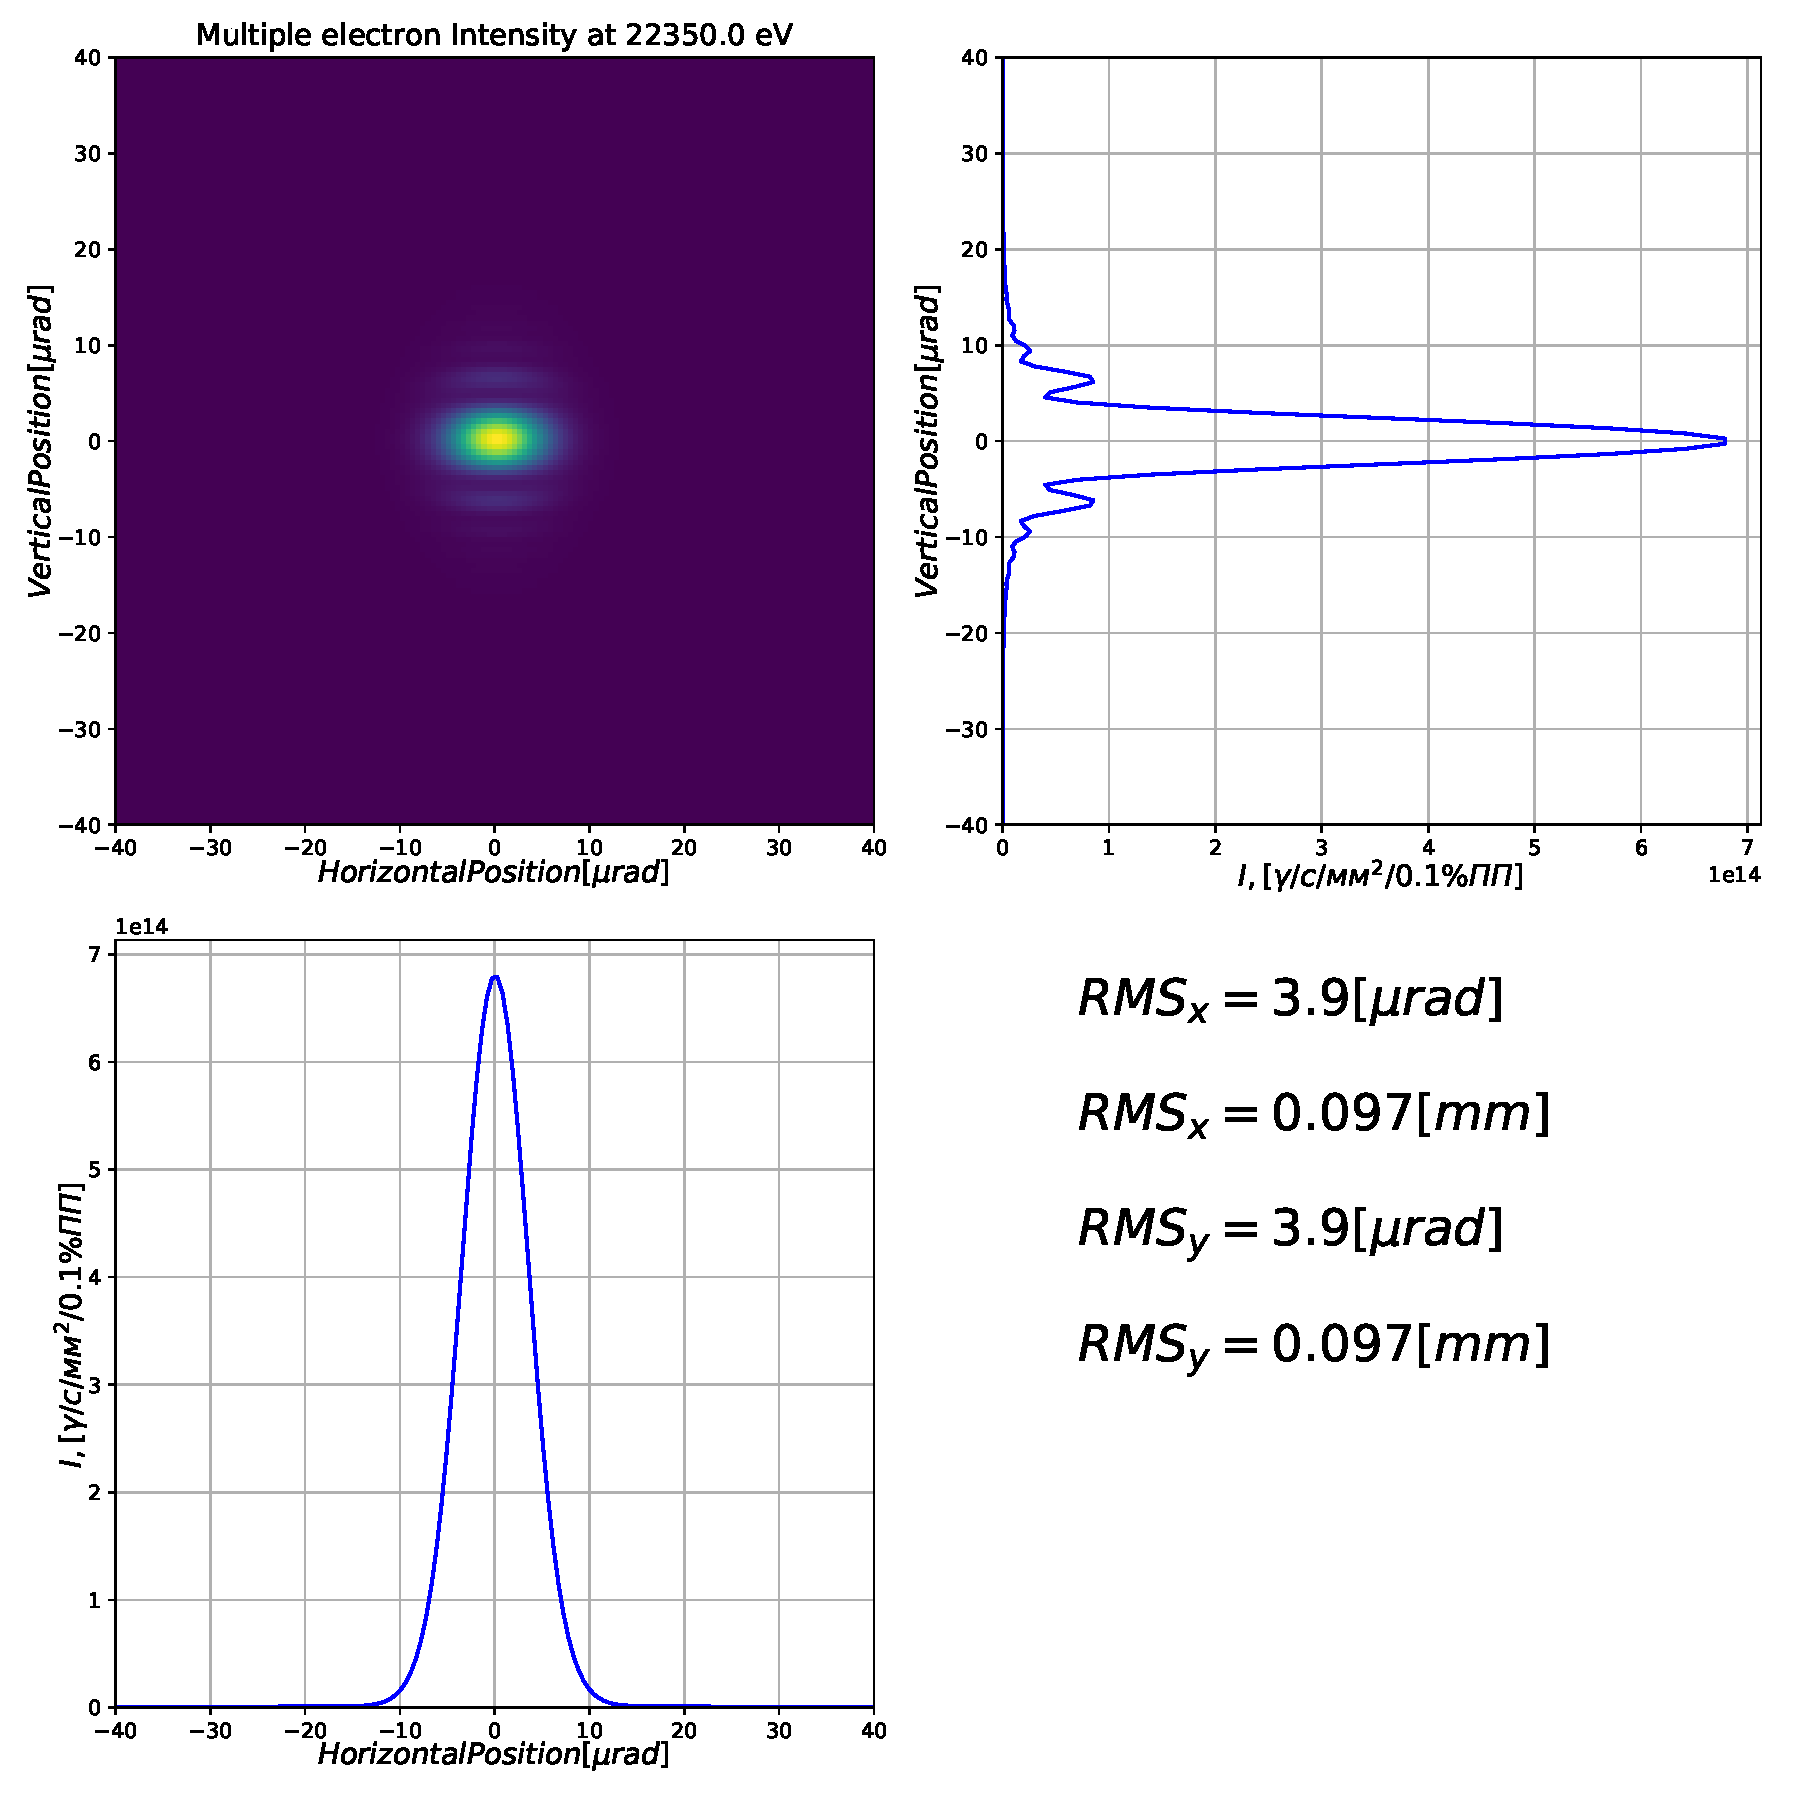
\includegraphics[width=\textwidth]{{pic/17_harm_before_crystal}.pdf}
		\end{minipage} 
		\begin{minipage}{0.49\textwidth}
			\centering
			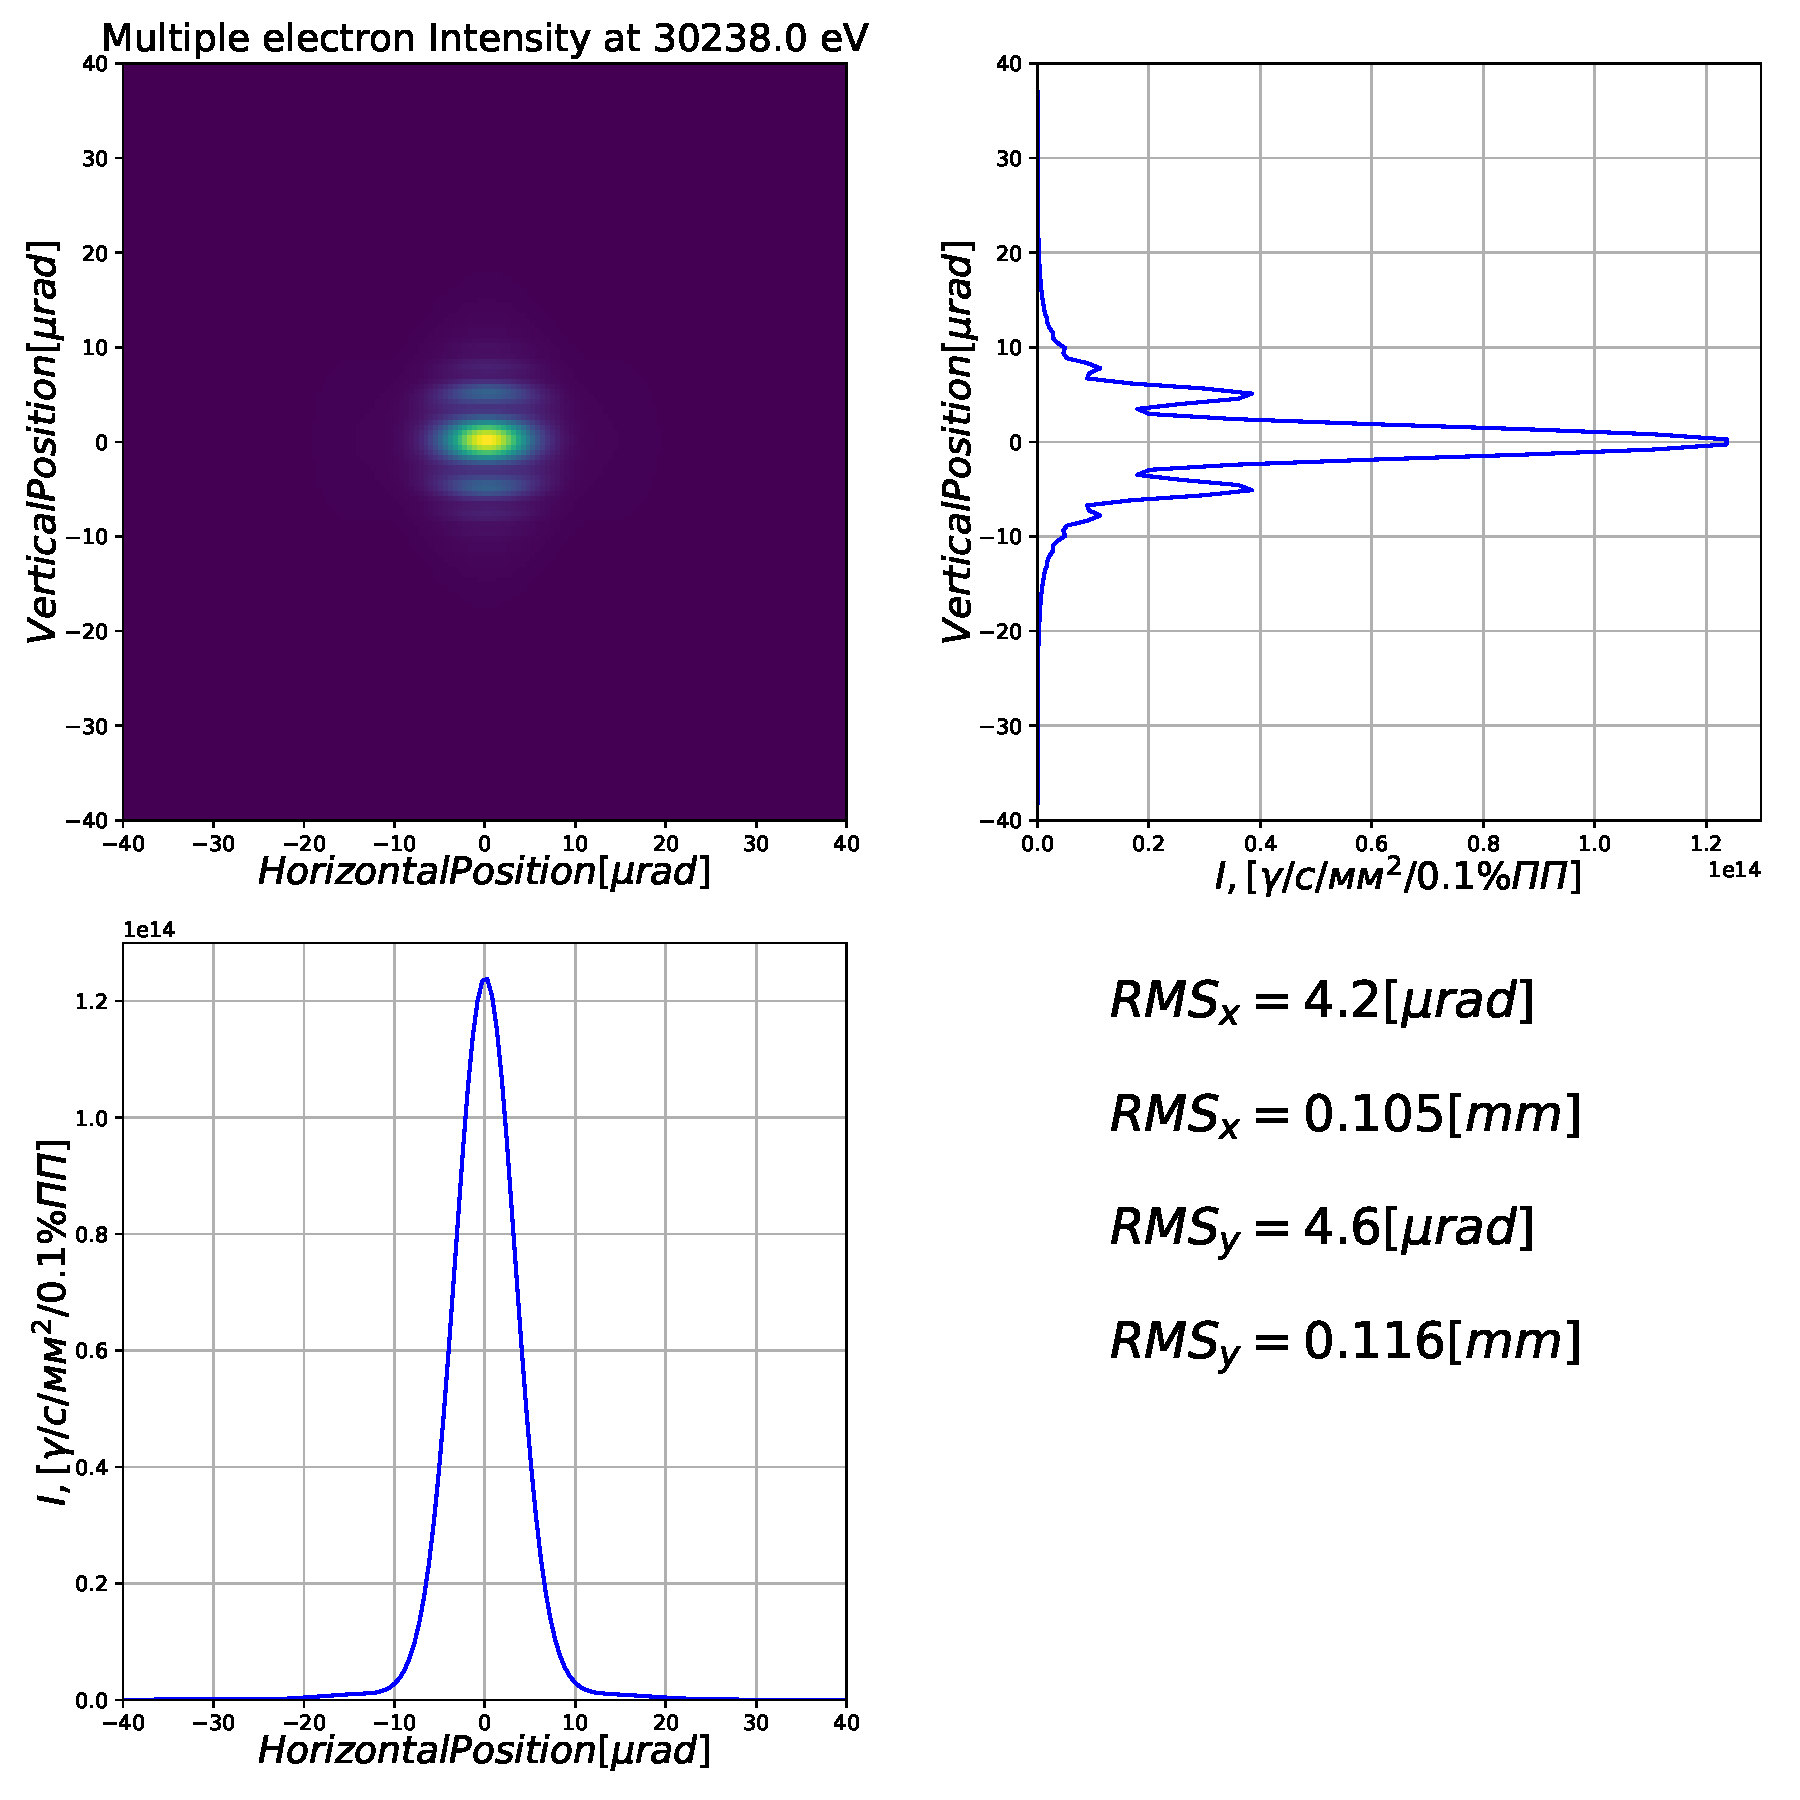
\includegraphics[width=\textwidth]{{pic/23_harm_before_crystal}.pdf}
		\end{minipage}
		\caption{Сечение пучка до первой аппретуры}    
		\label{fig:before_crystal}  
	\end{figure}
	
	\begin{figure}[htbp]
		\centering  
		\begin{minipage}{0.49\textwidth}
			\centering
			\includegraphics[width=\textwidth]{{pic/11_harm_after_crystal}.pdf}
		\end{minipage}\hfill
		\begin{minipage}{0.49\textwidth}
			\centering
			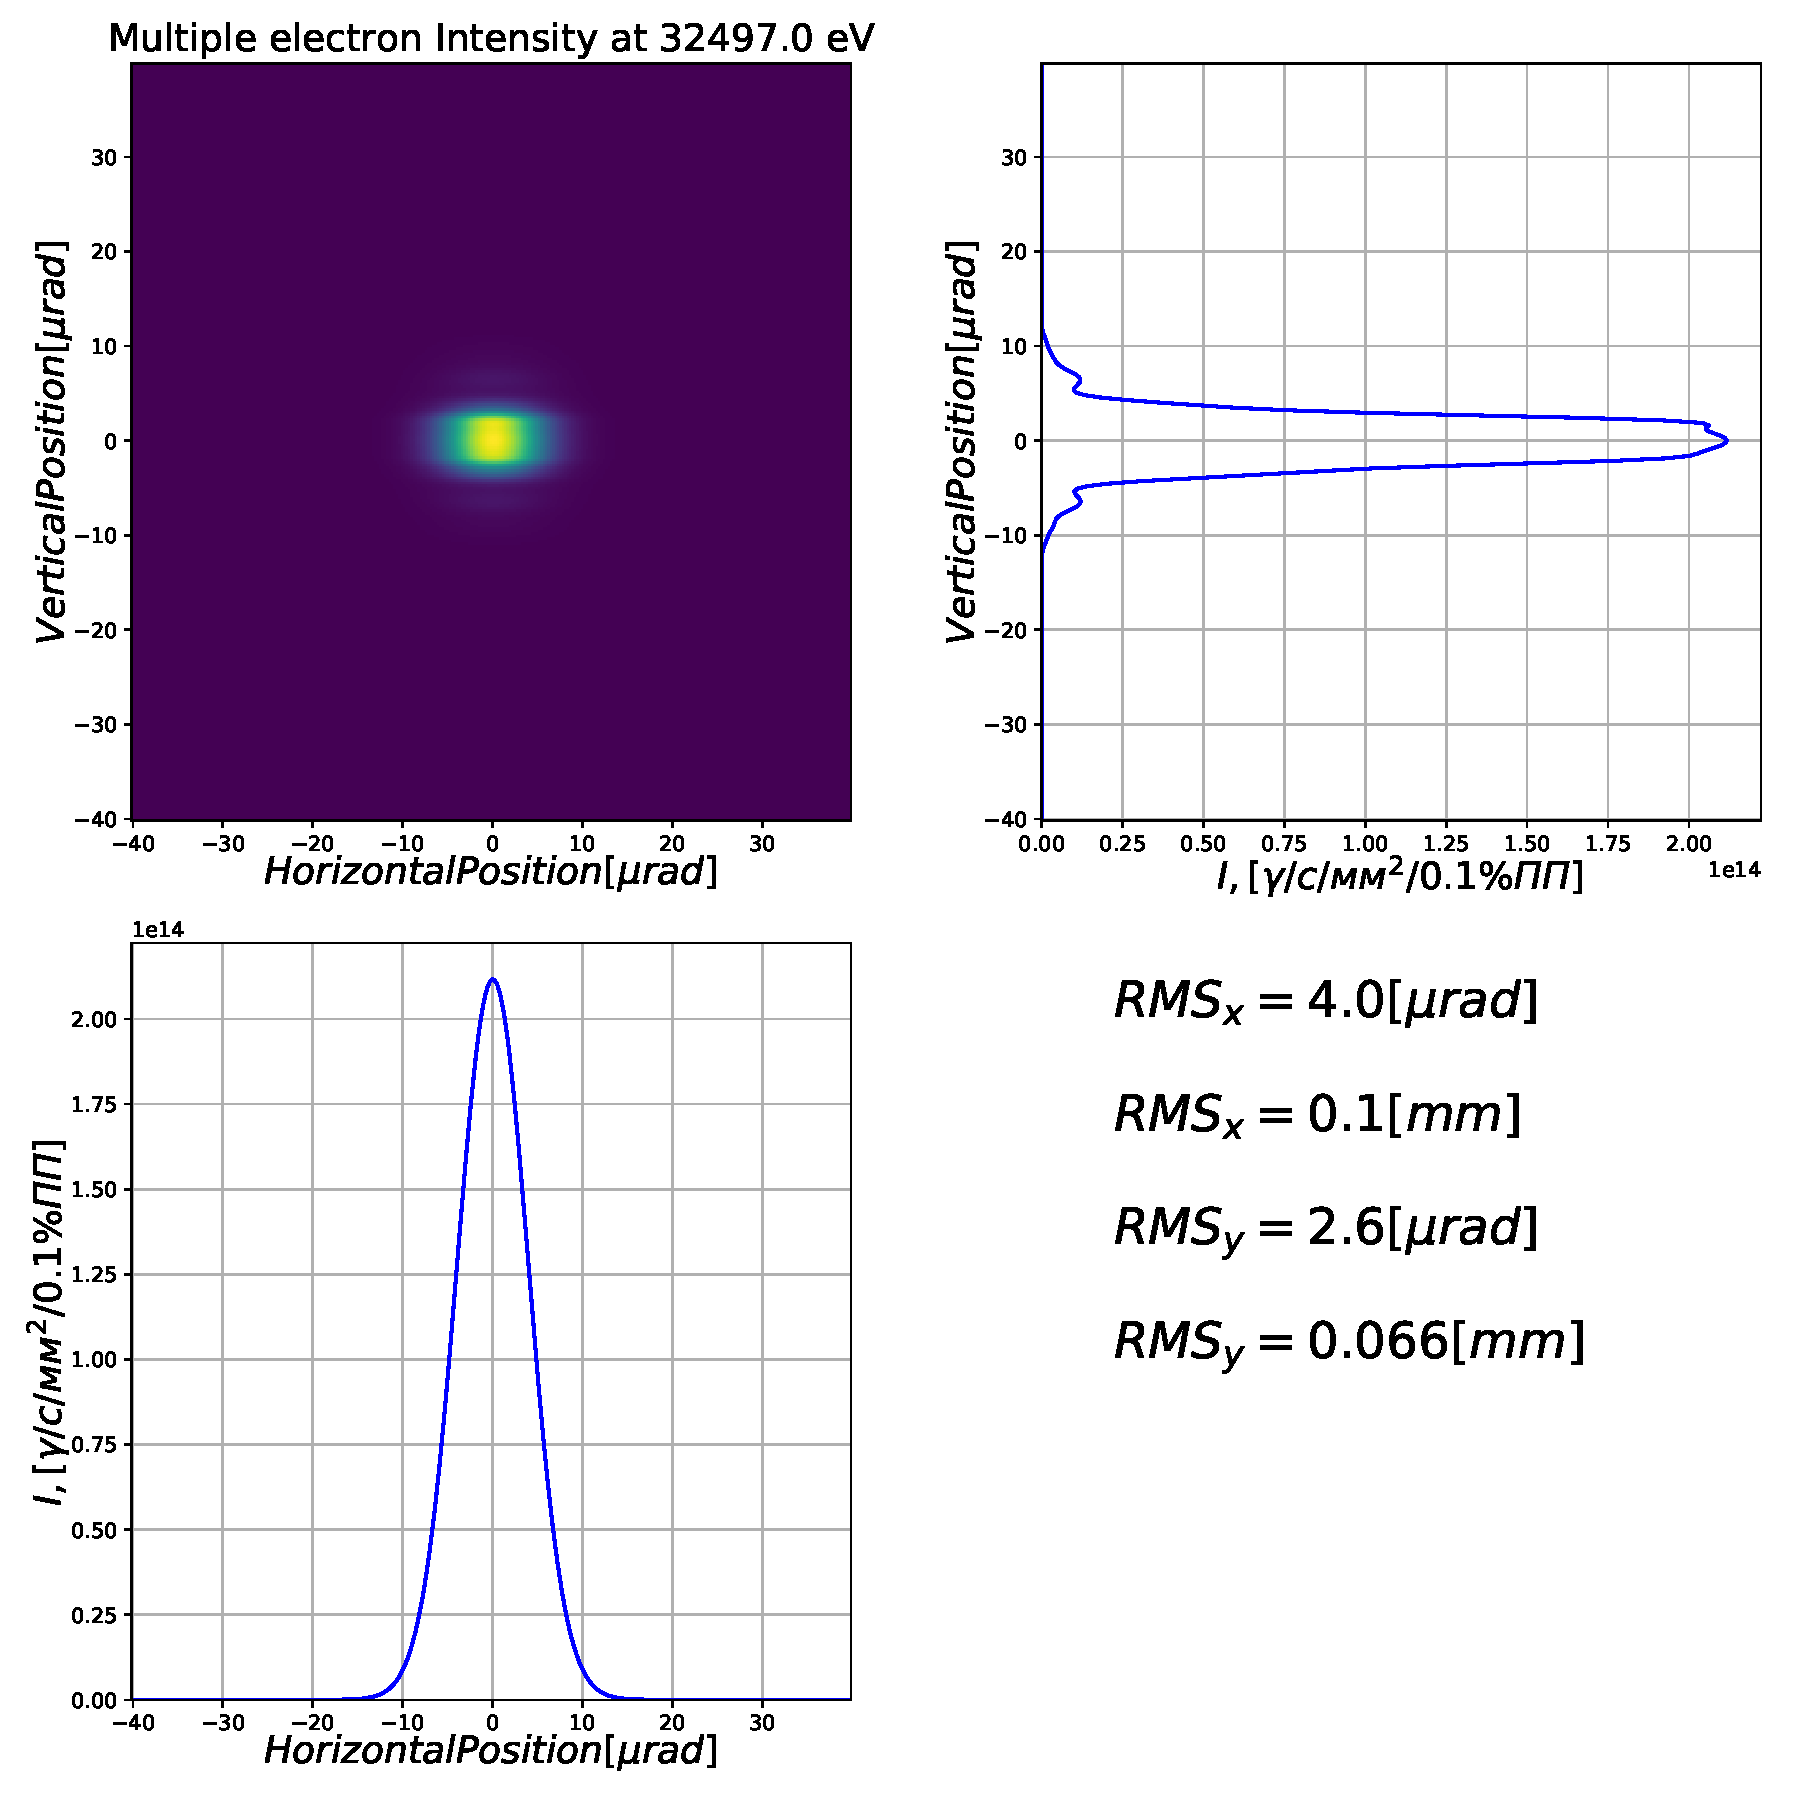
\includegraphics[width=\textwidth]{{pic/13_harm_after_crystal}.pdf}
		\end{minipage}
		\begin{minipage}{0.49\textwidth}
			\centering
			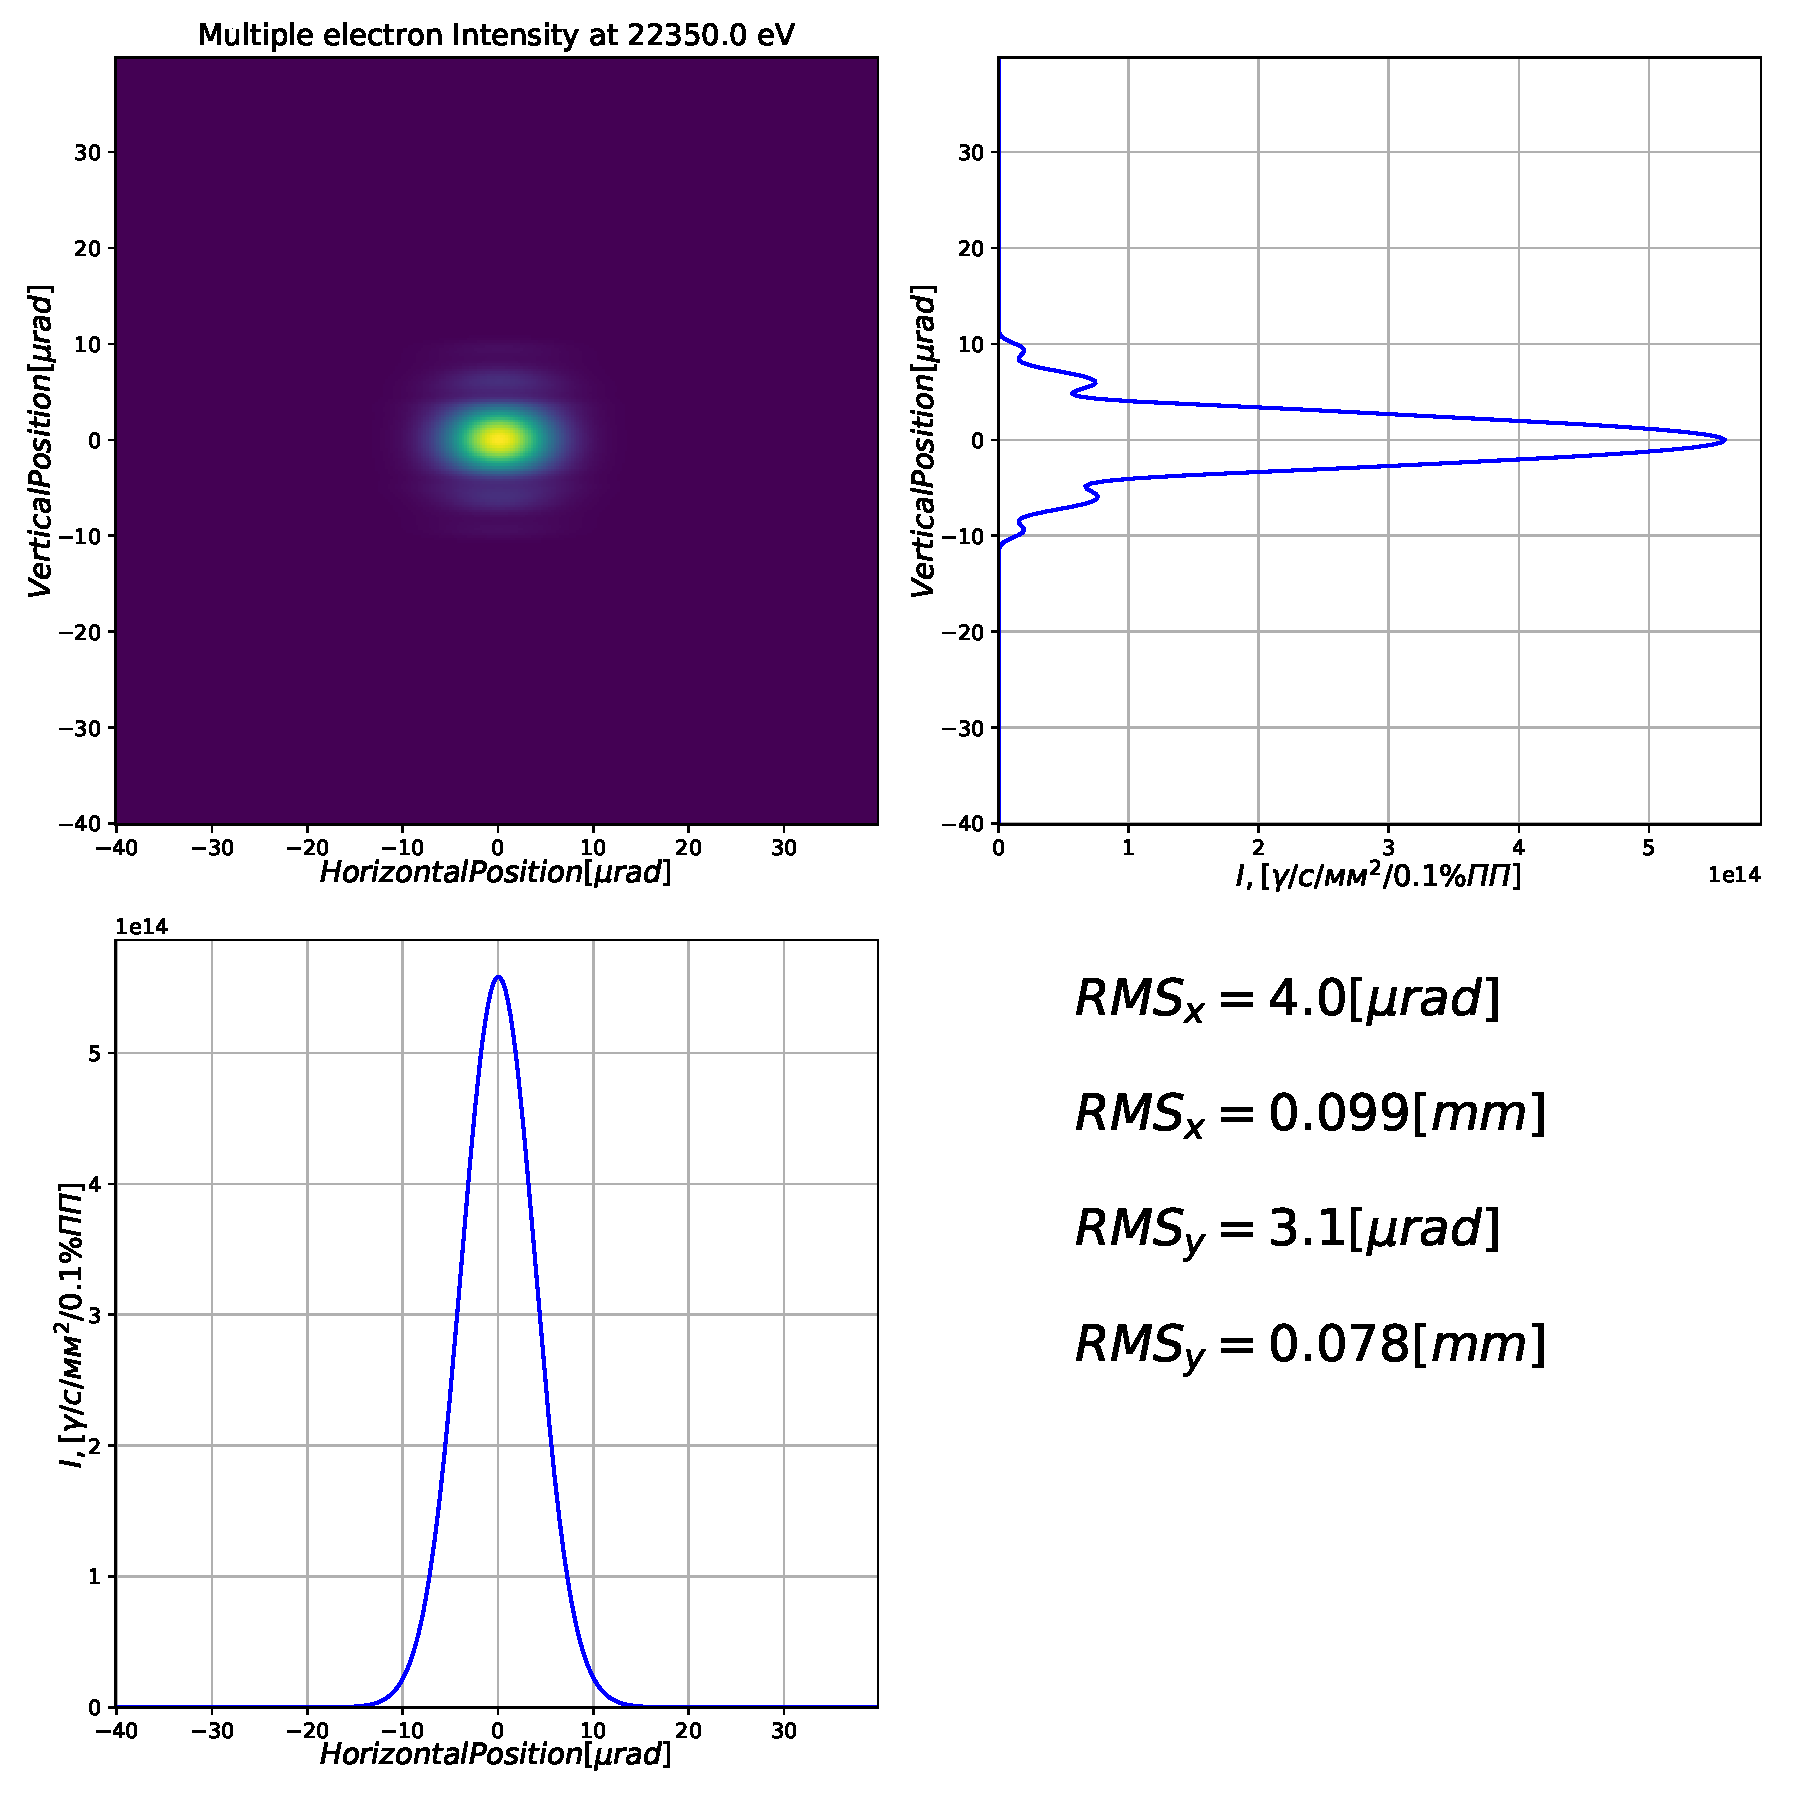
\includegraphics[width=\textwidth]{{pic/17_harm_after_crystal}.pdf}
			
		\end{minipage} 
		\begin{minipage}{0.49\textwidth}
			\centering
			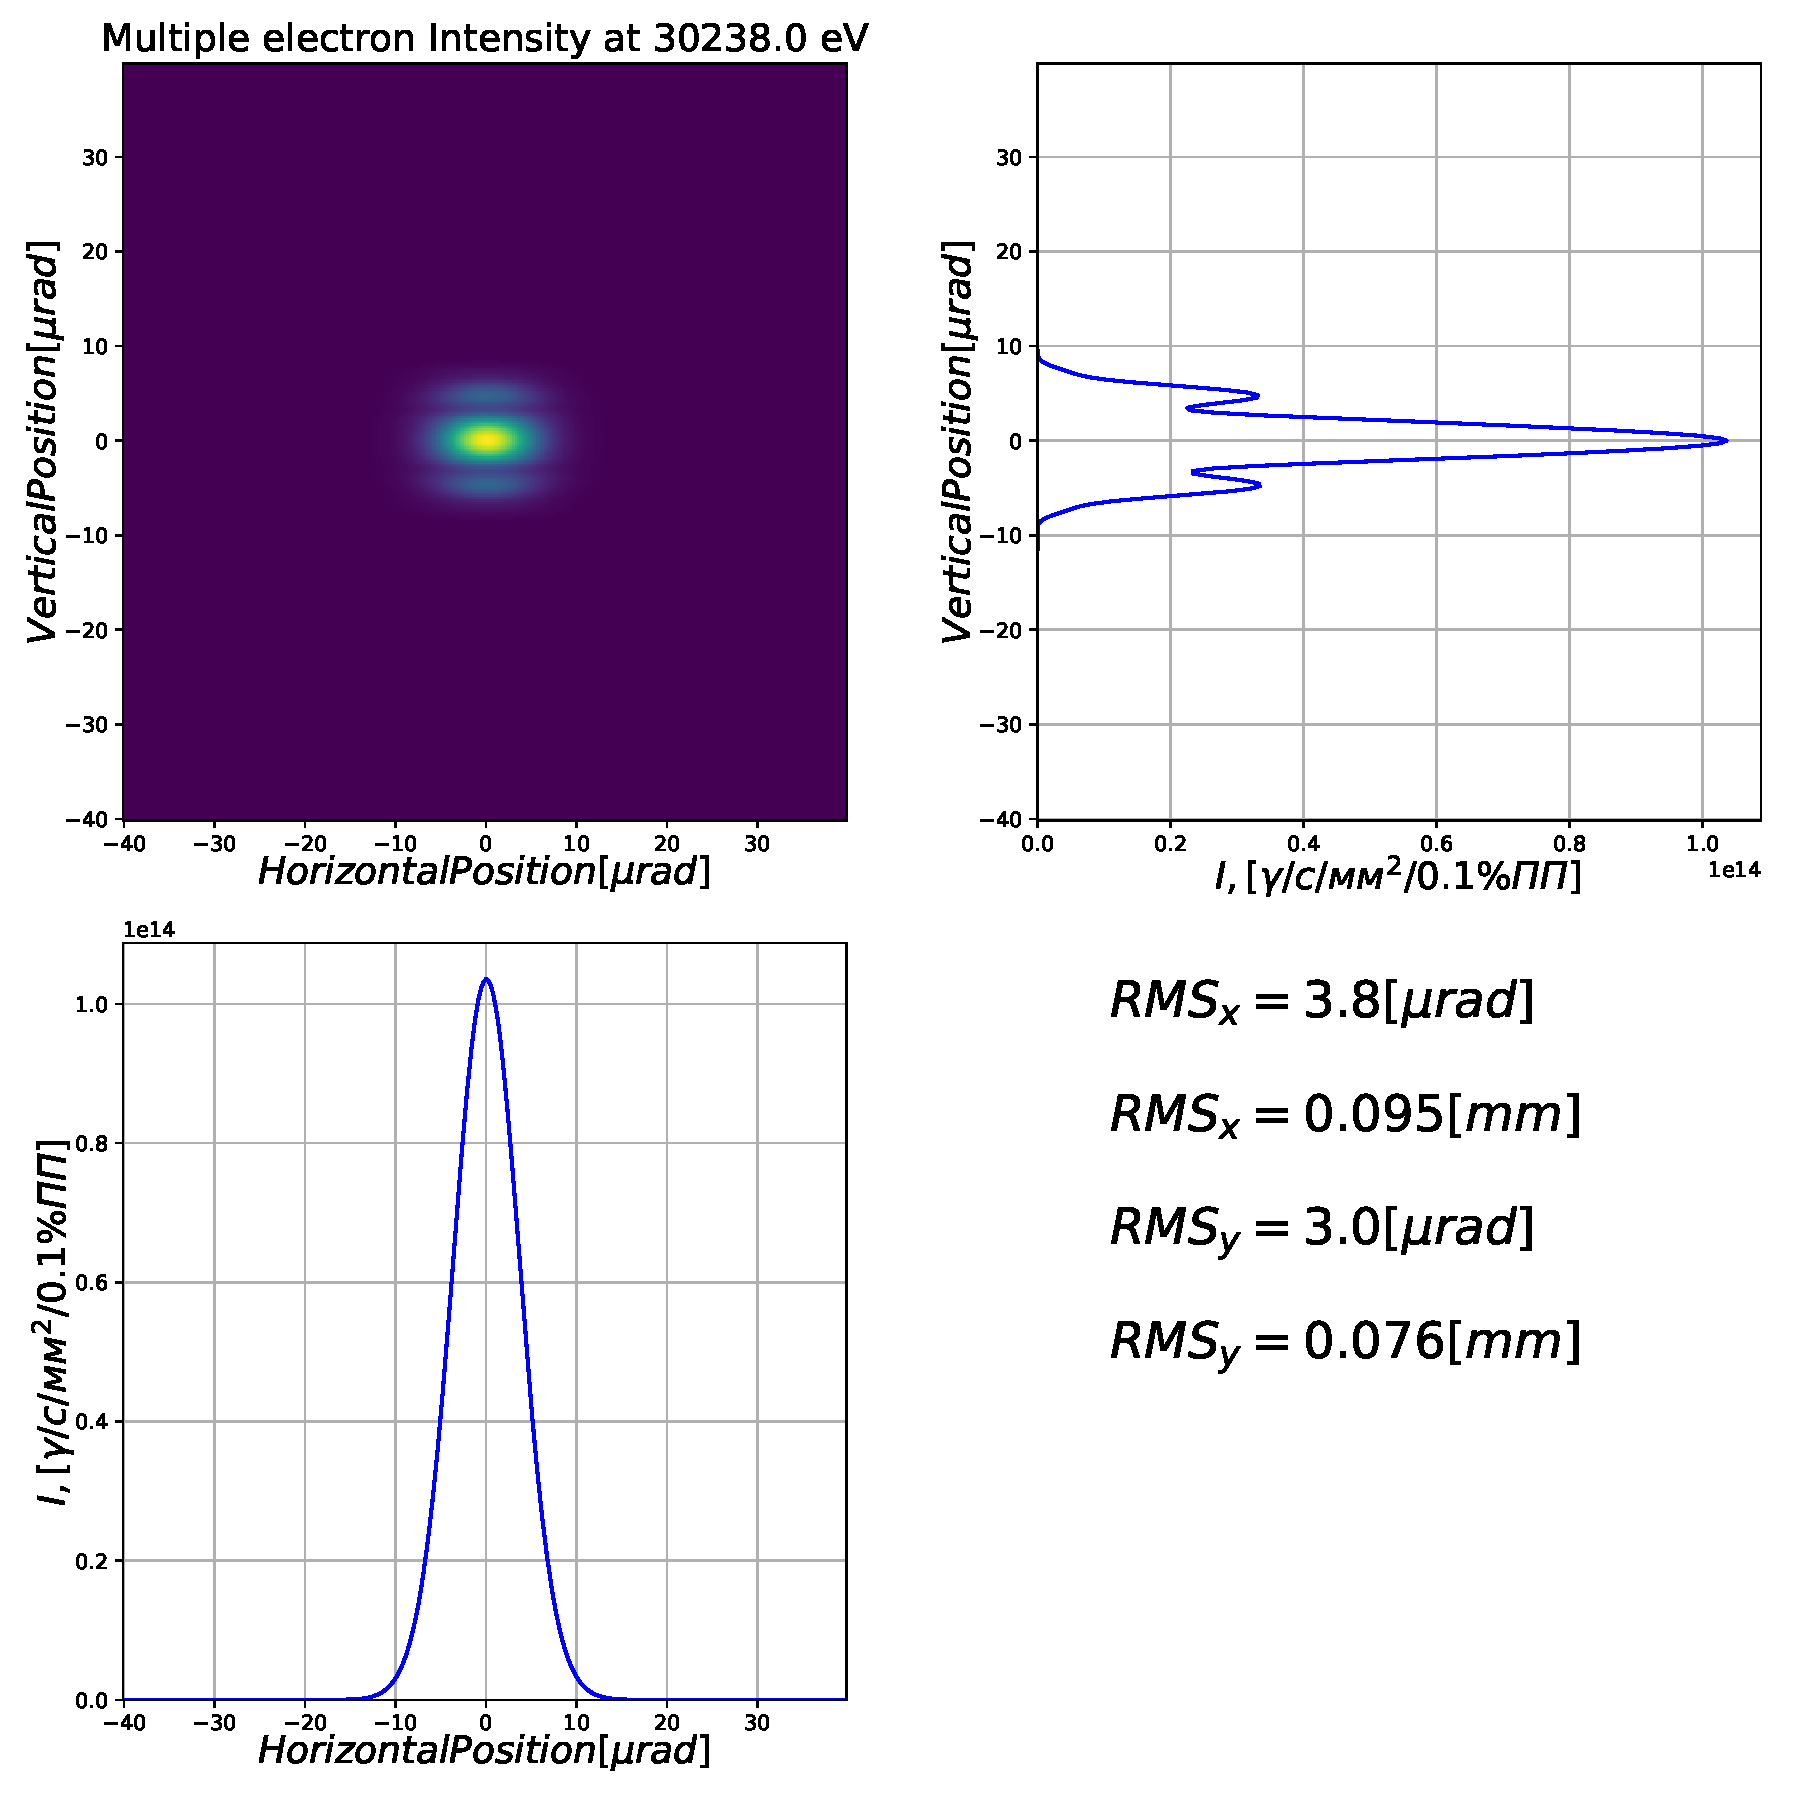
\includegraphics[width=\textwidth]{{pic/23_harm_after_crystal}.pdf}
		\end{minipage}
		\caption{Сечение пучка на выходе соответствующих монохроматоров}  
		\label{fig:after_crystal}  
	\end{figure}
	
	\begin{figure}[htbp]
	\centering  
	\begin{minipage}{1.\textwidth}
		\centering  
		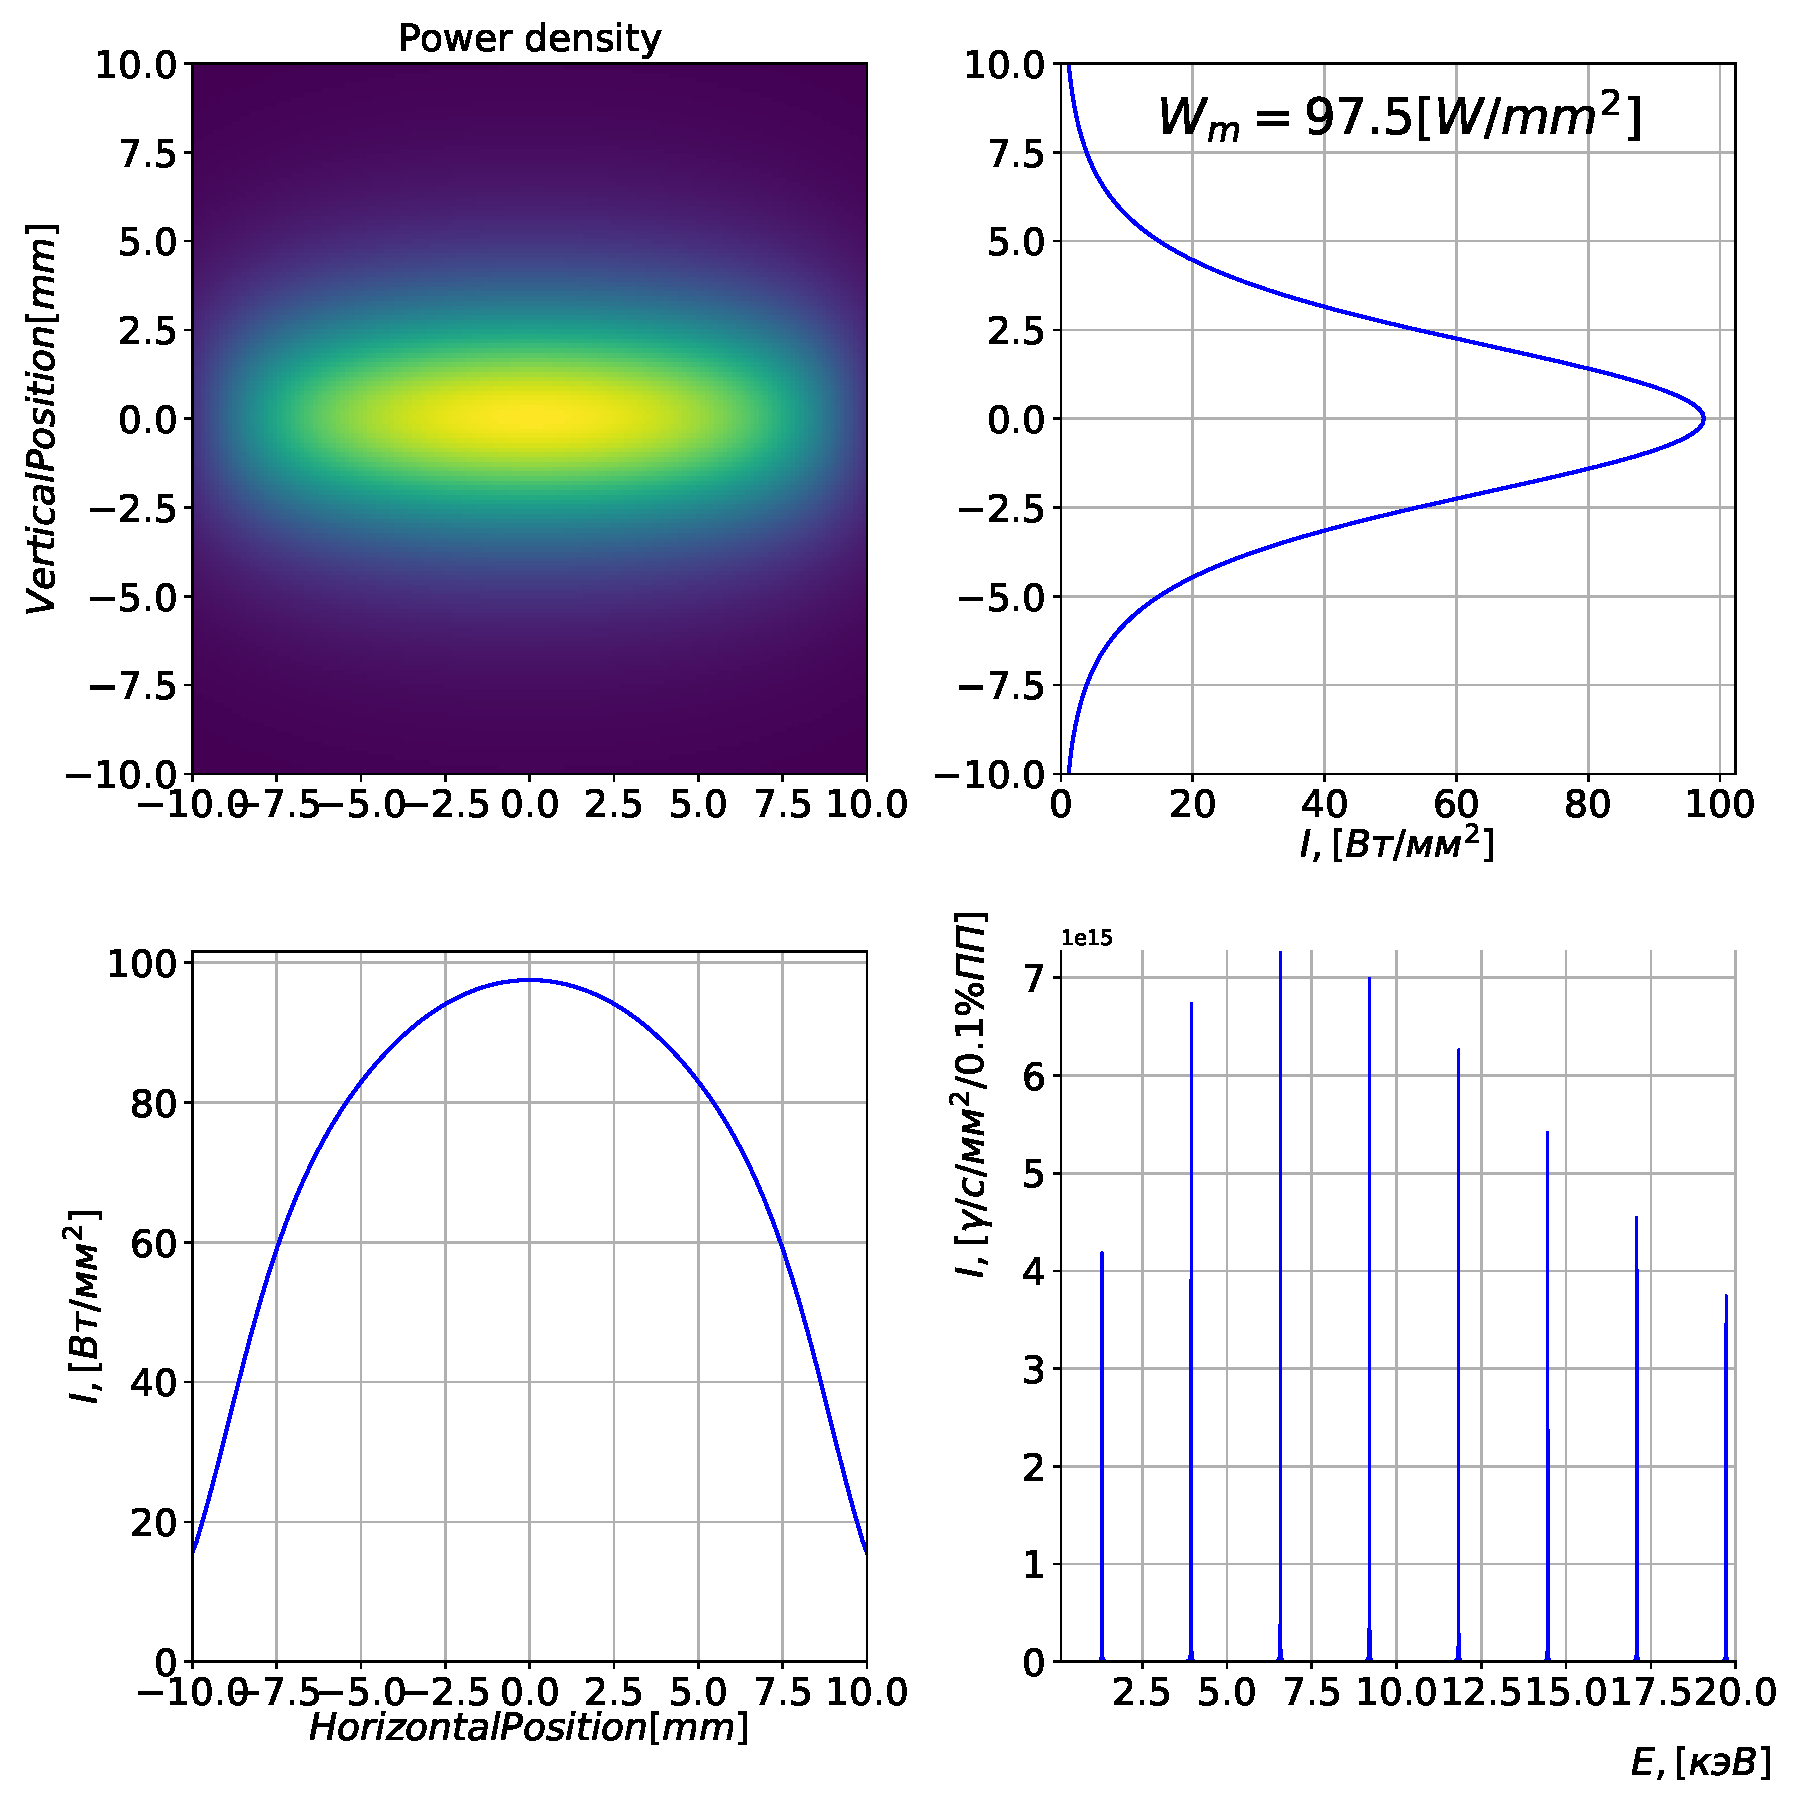
\includegraphics[width=\textwidth]{pic/power_dens.pdf}
		\caption{Плотность мощность и спектральная мощность источника}
		\label{fig:spec}
	\end{minipage}     
	\end{figure}

	
\end{document}



